% Scientific Reports submission (Springer Nature template, sn-nature reference style)
% Revised manuscript: method on measured outputs, biological/calibration split, re-estimation
% criterion, backward elimination, external validation, robustness, cost and formal guarantees.
% Figures: make_figures.py; Table 1 and Supplementary Table S1: make_tables.py.

\documentclass[pdflatex,sn-nature]{sn-jnl}

\usepackage{graphicx}
\usepackage{multirow}
\usepackage{amsmath,amssymb,amsfonts}
\usepackage{amsthm}
\usepackage{booktabs}
\usepackage{array}
\usepackage{xcolor}
\usepackage{url}
\usepackage{lineno}
\linenumbers
\raggedbottom

\theoremstyle{plain}
\newtheorem{theorem}{Theorem}

\makeatletter\def\toclevel@subparagraph{0}\makeatother % back-matter headings as top-level PDF bookmarks
\renewcommand{\floatpagefraction}{0.6}% allow float pages (Tables 1 and 2) that are not almost full
% DOI of the reproducibility package on Zenodo (replace after reserving it)
\newcommand{\zenododoi}{10.5281/zenodo.23338175}
\begin{document}

\title[Few biological parameters reproduce measured dynamics]{Few biological parameters suffice to reproduce measured dynamics in systems biology models: local sensitivity-based reduction with formal verification of the mathematical foundations}

\author*[1]{\fnm{M\'onica} \sur{Miranda R.}}\email{mmmirand@espol.edu.ec}
\author[1]{\fnm{Carlos} \sur{Salazar}}\email{asalazar@espol.edu.ec}
\author[1]{\fnm{C\'esar} \sur{Mart\'in}}\email{cmartin@espol.edu.ec}
\author[1]{\fnm{Adriana} \sur{Aguirre}}\email{aaaguirr@espol.edu.ec}

\affil*[1]{\orgdiv{Faculty of Engineering, Control and Automation Systems Group}, \orgname{Escuela Superior Polit\'ecnica del Litoral (ESPOL)}, \orgaddress{\city{Guayaquil}, \country{Ecuador}}}

\abstract{Mathematical models of biological processes often contain dozens to hundreds of unknown rate constants, but experimental data rarely contain enough information to estimate all of them. We present a method that, starting from published parameter values and before any new model fitting, identifies a small set of biological parameters sufficient to reproduce the measured data when only those parameters, together with the measurement scaling and offset factors, are re-estimated and all other parameters are kept at their published values. The method ranks parameters by how strongly they change the measured quantities, discards parameters whose effects are redundant, checks that the reduced model can reproduce the data under random parameter perturbations, and finally removes any parameter that is not needed. We applied it to 34 published models with real experimental data. In 32 of them, a small subset was sufficient, in most cases only two biological parameters. When fitted to part of the experiments, the reduced models predicted the remaining experiments as well as or better than the full models in 27 of 29 testable cases, and most remained adequate for parameter changes of up to 50\%. A leakage-free validation protocol confirmed that this result does not depend on the nominal parameter values having been estimated from the full data set. Two baseline controls---re-estimating only calibration parameters (no biological parameters) and selecting the same number of biological parameters at random---achieved similar test accuracy in most problems, consistent with the sloppy-model property; the exception was Oliveira, where the specific selection was more than 20-fold better than either control. The cost grows linearly with model size. Its main mathematical steps are verified with a computer proof assistant.}

\keywords{parameter reduction, practical identifiability, sensitivity analysis, ordinary differential equations, systems biology, formal verification}

\maketitle

% Scientific Reports: single-column text without justification
\raggedright
\setlength{\parindent}{1.5em}

\section*{Introduction}\label{sec:intro}\pdfbookmark[0]{Introduction}{bm1}

Ordinary differential equation (ODE) models are central to quantitative biology, pharmacology and epidemiology, where they describe how interacting molecular species or populations change over time as a function of kinetic parameters $\theta$\cite{bib16}. Using a model for prediction requires estimating $\theta$ from experimental measurements, and this becomes difficult as models grow. The main obstacle is non-identifiability: different parameter values may produce the same measured output, either because of model symmetries (structural non-identifiability) or because the available data are insufficient (practical non-identifiability)\cite{bib4,bib10,bib29}. In both cases the likelihood has flat ridges on which optimisers stall and confidence intervals become unreliable\cite{bib24,bib25,bib17}. Models in public benchmark collections routinely contain 20--300 parameters\cite{bib31}, and genome-scale models contain thousands\cite{bib12}.

The sloppy-model phenomenon offers a structural explanation\cite{bib15}: the sensitivity of model outputs to parameters is typically dominated by a few ``stiff'' directions, while many ``sloppy'' directions have almost no effect on the outputs. This suggests that a small subset of parameters may suffice to describe what is actually measured. Exploiting this observation in practice requires answering three questions that existing tools address only partially. First, which parameters should be retained? Sensitivity indices\cite{bib26,bib23} and profile likelihoods\cite{bib24} rank parameters by importance, but they do not ensure that the retained parameters are mutually non-redundant, so the reduced estimation problem may still be ill-conditioned\cite{bib5,bib9}. Second, is the reduced model good enough? A reduction is useful only if re-estimating the retained parameters reproduces the measured data and predicts experiments that were not used for fitting. Third, how much can the conclusions be trusted? Statements such as ``the discarded parameters can be fixed'' rest on approximations whose validity is rarely made explicit.

This work was motivated by a dynamical model of Bandura's social cognitive theory\cite{bib3,bib34}, in which six psychosocial constructs that determine physical activity interact through 22 parameters (coupling strengths, input gains and time constants). When all 22 parameters were estimated from 31 days of step-count data, many stable parameter sets fitted the data with widely different quality (coefficients of determination between 4\% and 86\%), and local refinement from the best global estimate lowered the fit from 86\% to 41\%\cite{bib35}. Such behaviour is typical when several parameters have nearly identical effects on the measured output, so that the data cannot separate them; in such models, a principled way to decide which parameters to estimate is indispensable.

Here we present a reduction method that works directly on the measured outputs defined in the PEtab format\cite{bib27}, including experimental conditions, measurement transformations and noise levels. It distinguishes biological parameters, which belong to the mechanistic model, from calibration parameters (scaling factors and offsets of the measurement process), which are always re-estimated, and selects only among the biological ones. Candidates are ranked by sensitivity, redundant candidates are rejected by condition-number and variance-inflation tests, the reduced model is accepted only if re-estimating its parameters reproduces the full model under random parameter perturbations, and a final backward elimination makes the subset minimal with respect to inclusion. We evaluate the method on 34 benchmark problems with real data\cite{bib31,bib27}, test the reduced models on held-out experiments, quantify their robustness to perturbation size and to the method's own settings, and report the computational cost. The main mathematical statements on which the method relies are formally verified in the Lean~4 proof assistant with the Mathlib library\cite{bib19,bib21}; we state precisely what is and what is not proved.

\section*{Results}\label{sec:results}\pdfbookmark[0]{Results}{bm2}

\subsection*{Overview of the method}\label{sec:overview}\pdfbookmark[1]{Overview of the method}{bm3}

Figure~\ref{fig:pipeline} summarises the procedure; all symbols are defined in the Methods and in Supplementary Table~S2 (Supplementary Note \textit{Notation of the method}). The input is a PEtab problem: an SBML model, the list of measured observables with their experimental conditions, measurement times, transformations (linear, logarithmic) and noise standard deviations $\sigma_i$, and the nominal parameter values $\theta_0$ reported by the original authors. Each measurement $i$ defines a scaled output $y_i(\theta)=h(g_i(x(t_i;\theta),\theta))/\sigma_i$, so that all outputs are comparable in units of measurement noise. Parameters are split into biological parameters $\theta_B$ (those of the SBML model) and calibration parameters $\theta_C$ (observation scalings and offsets); only biological parameters are candidates for selection, while calibration parameters are always re-estimated together with the selected ones.

The relative sensitivity matrix $J=\partial y/\partial\log\theta$ is computed once at $\theta_0$ by central finite differences. In stage~1, biological parameters are added in decreasing order of their sensitivity energy $E_j=\|J_{:,j}\|^2$; a candidate is accepted only if the condition number $\kappa$ and the largest variance inflation factor (VIF) of the normalised columns of $J_S$ stay below a threshold, and is otherwise discarded permanently. Stage~1 stops when the accepted parameters capture a fraction $\tau_R$ of the total energy. The resulting subset $S$ is then tested: in random scenarios where all parameters are perturbed, $\theta_S$ and $\theta_C$ are re-estimated with the remaining parameters fixed at $\theta_0$, and $S$ is admissible if the median relative fitting error $e_{\mathrm{fit}}$ is below $\tau_e$ and $|S|\ge 2$. The threshold $\tau_e=\sqrt{1-c^2}$ equals the smallest error attainable by rescaling an output change whose cosine similarity with the full change is $c$ (Theorem~\ref{thm:cos}); we use $c=0.9$, so $\tau_e=0.436$. If stage~1 does not yield an admissible subset, stage~2 repeats the selection with parameters ordered by their finite-perturbation effect $s_j$ until an admissible subset is found. Finally, backward elimination removes any parameter whose removal keeps the subset admissible, which yields a subset that is minimal with respect to inclusion (Theorem~\ref{thm:prune}).

\begin{figure}[t]
\centering
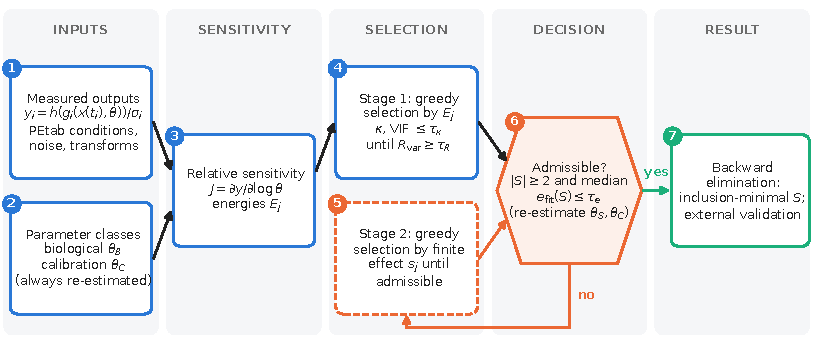
\includegraphics[width=\textwidth]{figures/fig1_pipeline.pdf}
\caption{\textbf{Overview of the reduction method.} Biological parameters are ranked by their effect on the measured outputs and selected with conditioning control ($\kappa$ and VIF thresholds; stage~1, or stage~2 if needed, dashed). A subset is accepted when re-estimating it reproduces the full model; backward elimination then makes it minimal, and the reduced model is validated on held-out data.}
\label{fig:pipeline}
\end{figure}

\subsection*{A motivating case with exact collinearity}\label{sec:sct}\pdfbookmark[1]{A motivating case with exact collinearity}{bm4}

The social cognitive theory model\cite{bib3,bib34,bib35} describes six psychosocial constructs through a linear system with 22 parameters and a single measured output (daily steps from one participant\cite{bib35}). At the published estimate $\theta_0$, the sensitivity matrix of behaviour is exactly rank-deficient (infinite condition number, maximum VIF $4.5\times10^{15}$), with nine pairs of parameters having cosine similarity above 0.95, making the full estimation problem ill-posed. The method selected two parameters ($\gamma_{57}$ and $\beta_{45}$, the path from the external input through social satisfaction to behaviour), which, re-estimated on days 1--24, predicted the held-out week with $R^2=0.84$ (test $\chi^2/n$ 1.63), better than the full model refitted locally ($R^2=0.67$) or by differential evolution ($R^2=0.79$); the model is not counted in the benchmark statistics below (Supplementary Note \textit{\nt{sct}}, Supplementary Table~S18 and Supplementary Fig.~S5).

\subsection*{Benchmark: a few biological parameters suffice in most models}\label{sec:benchmark}\pdfbookmark[1]{Benchmark: a few biological parameters suffice in most models}{bm5}

We applied the method to 34 PEtab benchmark problems with real measurements\cite{bib31,bib27} covering signalling, metabolism, gene regulation, cell cycle, immunology and epidemiology, with 3 to 294 parameters and 16 to 27,132 measurements (Table~\ref{tab:benchmark}); Supplementary Note \textit{System-by-system summary} describes each problem, the meaning of its selected parameters and its validation. One further benchmark problem (Froehlich, 4,231 parameters and 9,169 experimental conditions) was analysed only on its state trajectories because each evaluation of its measured outputs requires about 9,000 simulations; it is not counted here (see Computational cost).

The method found an admissible subset in 32 of the 34 problems (Fig.~\ref{fig:benchmark} and Table~\ref{tab:benchmark}). In 29 of them the subset contains only two biological parameters; two is also the minimum subset size enforced by the method ($k_{\min}=2$), so this result does not imply that a single parameter would be insufficient---Supplementary Note \textit{\nt{single}} shows that one biological parameter already reaches the admissibility threshold in 16 of 27 tested problems. The remaining three subsets contain three (Zhao), five (Bruno) and ten (Lucarelli) biological parameters. Sixteen problems also have calibration parameters (up to 79 in Raimundez), which are re-estimated in every case. Counting both kinds, the reduced estimation problem has a median of 78\% fewer free parameters than the full one (range 33--97\%); among biological parameters alone, the median reduction is 88\%. Backward elimination removed between one and five parameters in seven problems (Supplementary Note \textit{Selected subsets of the benchmark problems}, Supplementary Table~S1). All 32 subsets satisfy the conditioning thresholds ($\tau_\kappa=\tau_{\mathrm{VIF}}=10$; maximum observed $\kappa=6.6$, VIF$=9.9$), which bound the uniqueness and stability of the linearised least-squares estimates of the retained parameters (Supplementary Table~S3, step~7) but do not require orthogonality; some selected pairs have cosine similarity near 0.9. Besides the admissibility condition $e_{\mathrm{fit}}\le\tau_e$, which all of them meet, 18 subsets also have a median $\cos\Delta\ge0.9$, so that a single rescaling of the reduced response already achieves the threshold (Theorem~\ref{thm:cos}), and two of these (Alkan and Perelson) also keep at least 89\% of the sensitivity energy, so that the first-order error bound applies as well; Supplementary Table~S1 gives these levels of guarantee for every problem. A low $R_{\mathrm{var}}$ or $\cos\Delta$ does not prevent a good reduction, because the re-estimated parameters compensate for the effects of the fixed ones. In Raimundez (79 calibration parameters) the median $\cos\Delta=-0.30$ is negative, meaning the two selected biological parameters move the outputs in a direction opposed to the total sensitivity; the calibration parameters nonetheless achieve $e_{\mathrm{fit}}=0.37<\tau_e$, placing this problem in the calibration-dominated category confirmed by the controls (Supplementary Table~\ref{tab:controls}). The cosine criterion (Theorem~\ref{thm:cos}) is a sufficient but not necessary condition for admissibility. Stage~1 alone was sufficient in seven problems; in the other 25, the energy ordering selected parameters whose re-estimation could not reproduce the full model, and the finite-effect ordering of stage~2 was needed. The two non-admissible problems fail for different reasons. In Crauste, a model of the T-cell response with quadratic proliferation and pathogen-growth terms, the published parameters lie at the edge of a regime in which the solution grows without bound in finite time. With the published parameters the effector populations rise to about $10^6$ cells near day 10 and then decline; after a change of only 1\% in a single parameter (for example, a decrease of the effector proliferation rate $\rho_E$) they keep growing and the solution breaks down between days 8.8 and 9.9, well within the measured horizon of 28 days. This happened for 8--9 of the 24 one-at-a-time perturbations of $\pm$1\% and for 7 of the 15 scenarios at $\pm$5\%, independently of the integrator tolerances (relative tolerances from $10^{-10}$ to $10^{-5}$), so the sensitivity matrix and the admissibility test are not defined and no local reduction method is applicable; consistently, global existence of solutions for this model could only be proved formally on a short horizon ($T\le 1$). In Beer, the selection stopped at 18 parameters because any further parameter violated the conditioning test, and the resulting subset had $e_{\mathrm{fit}}=50\%$, above the threshold.

Re-estimation is essential. When the selected parameters are simply set to their perturbed values, without re-estimation, the median relative error $e_{\mathrm{rel}}$ exceeds $\tau_e$ in 23 of the 32 admissible problems (Fig.~\ref{fig:benchmark}b); after re-estimation the median error $e_{\mathrm{fit}}$ is 14\% (maximum 43.5\%). In other words, the selected parameters do not replicate the effect of every individual perturbation; rather, adjusting them compensates for the perturbations of all other parameters in the measured outputs. This is precisely the property needed when the reduced model is fitted to data.

\begin{figure}[p]
\centering
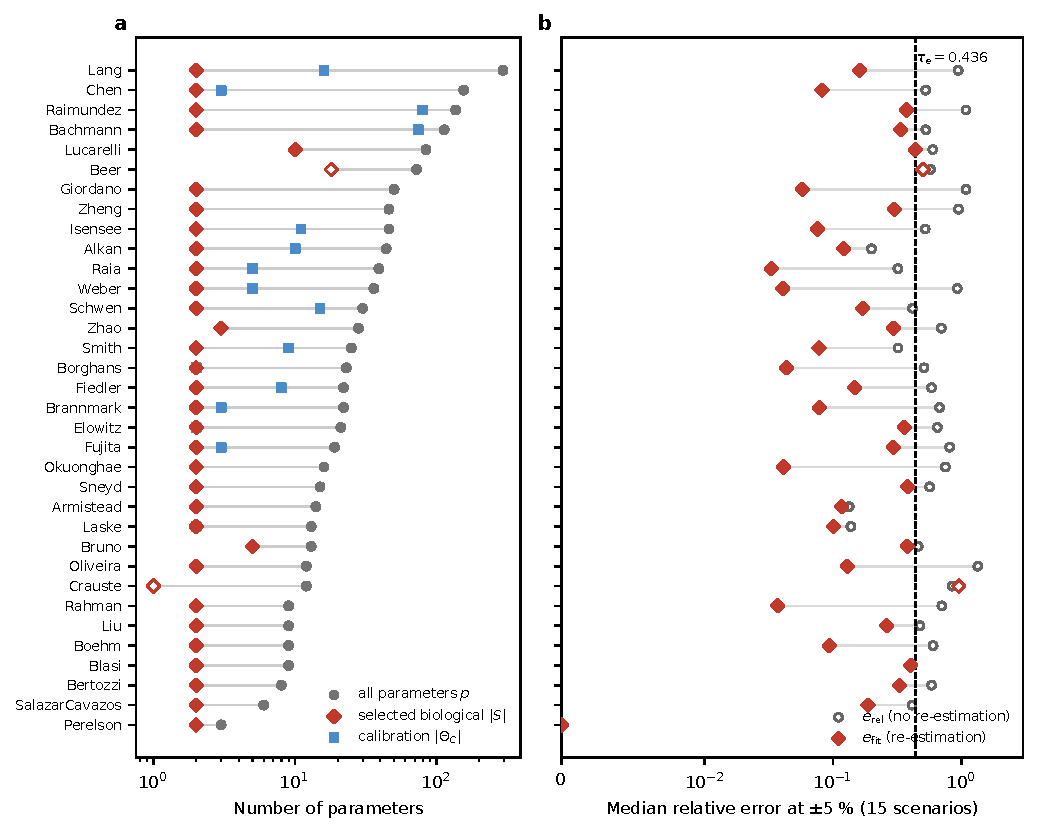
\includegraphics[width=\textwidth,height=0.8\textheight,keepaspectratio]{figures/fig2_benchmark.pdf}
\caption{\textbf{Parameter reduction and recovery of the full-model output in 34 benchmark problems.} Problems are ordered by the reduction achieved; the two without an admissible subset are at the bottom. \textbf{a}, Estimated parameters of the full model ($p$, grey) and parameters re-estimated in the reduced model (selected biological plus calibration parameters, blue). \textbf{b}, Median relative error over 15 random scenarios at $\pm$5\% before ($e_{\mathrm{rel}}$, open circles) and after re-estimating the retained parameters ($e_{\mathrm{fit}}$, green; stars, first-order estimate). The shaded region is the admissible region, $e_{\mathrm{fit}}\le\tau_e=43.6\%$.}
\label{fig:benchmark}
\end{figure}

\begin{table}[p]
\caption{\textbf{Per-problem results.} $p$, number of estimated parameters; $m$, number of measurements; $|\Theta_C|$, calibration parameters (always re-estimated); $|S|$, selected biological parameters; Stage, stage that produced the subset; $e_{\mathrm{rel}}$ and $e_{\mathrm{fit}}$, median relative error over 15 scenarios at $\pm$5\% without and with re-estimation (admissibility: $e_{\mathrm{fit}}\le 43.6\%$; italic, not admissible; $^{\ast}$, $e_{\mathrm{fit}}$ computed to first order because of simulation cost; $^{\dagger}$, not defined because the model has no solution on the measured horizon for 1\% parameter changes); Pattern, behaviour of the median $e_{\mathrm{fit}}$ for perturbation sizes from $\pm$1\% to $\pm$50\% (A, admissible at all sizes; B, admissible up to at least $\pm$20\% and not beyond; C, irregular; D, not admissible at $\pm$10\% or less; --, not applicable); Test $\chi^2/n$, mean squared noise-scaled residual on held-out experiments for the reduced and the full model, both re-estimated on the training experiments (values near 1 mean errors of the size of the measurement noise; --, not evaluable or not run).}
\label{tab:benchmark}
\centering
\scriptsize
\setlength{\tabcolsep}{4pt}
\begin{tabular}{@{}lrrrrcrrcccc@{}}
\toprule
System & $p$ & $m$ & $|\Theta_C|$ & $|S|$ & Stage & $e_{\mathrm{rel}}$ & $e_{\mathrm{fit}}$ & Level & Pattern & Ident. & Test $\chi^2/n$ \\
 & & & & & & (\%) & (\%) & & & (Lean) & red. / full \\
\midrule
Alkan & 44 & 1733 & 10 & 2 & 1 & 20 & 12.0$^{\ast}$ & 3 & A & 2/2 (1) & 2.75 / 3.37 \\
Armistead & 14 & 58 & 0 & 2 & 2 & 60 & 33.0 & 1 & B & 2/2 (2) & 1.22 / 1.37 \\
Bachmann & 113 & 541 & 74 & 2 & 2 & 53 & 33.8$^{\ast}$ & 1 & A & 2/2 (0) & 4.77 / 7.35 \\
Beer & 72 & 27132 & 0 & 18 & 2 & 57 & \textit{50.1$^{\ast}$} & -- & -- & -- & -- \\
Bertozzi & 8 & 22 & 0 & 2 & 2 & 58 & 32.9 & 2 & B & 2/2 (0) & -- \\
Blasi & 9 & 252 & 0 & 2 & 1 & 41 & 40.2 & 2 & B & 2/2 (2) & -- \\
Boehm & 9 & 48 & 0 & 2 & 2 & 60 & 9.4 & 2 & A & 2/2 (2) & 2.57 / 11.22 \\
Borghans & 23 & 111 & 2 & 2 & 2 & 51 & 4.3 & 1 & A & 2/2 (0) & 0.74 / 0.74 \\
Brannmark & 22 & 43 & 3 & 2 & 2 & 67 & 7.8 & 1 & A & 2/2 (0) & 5.96 / 6{,}277 \\
Bruno & 13 & 77 & 0 & 5 & 1 & 46 & 37.8 & 2 & A & 5/5 (5) & 0.91 / 208 \\
Chen & 155 & 120 & 3 & 2 & 2 & 53 & 8.1$^{\ast}$ & 1 & A & 2/2 (0) & 20.88 / 17.71 \\
Crauste & 12 & 21 & 0 & -- & 2 & -- & \textit{n.d.}$^{\dagger}$ & -- & -- & -- & -- \\
Elowitz & 21 & 58 & 2 & 2 & 1 & 65 & 35.8 & 1 & B & 2/2 (0) & 1.50 / 3.89 \\
Fiedler & 22 & 72 & 8 & 2 & 2 & 58 & 14.7 & 1 & A & 2/2 (0) & 11.21 / 9.32 \\
Fujita & 19 & 144 & 3 & 2 & 2 & 81 & 29.4 & 1 & A & 0/2 (0) & 5.94 / 8.03 \\
Giordano & 50 & 313 & 0 & 2 & 2 & 108 & 5.8 & 2 & A & 0/2 (0) & $<$0.01 / $<$0.01 \\
Isensee & 46 & 687 & 11 & 2 & 1 & 52 & 11.3$^{\ast}$ & 1 & A & 2/2 (0) & 1.08 / 1.08 \\
Lang & 294 & 9600 & 16 & 13 & 2 & 70 & \textit{56.4$^{\ast}$} & -- & -- & -- & -- \\
Laske & 13 & 42 & 2 & 2 & 1 & 14 & 10.1 & 2 & A & 2/2 (1) & 0.76 / 1.87 \\
Liu & 9 & 100 & 0 & 2 & 2 & 47 & 26.1 & 2 & A & 2/2 (0) & 0.95 / 1.02 \\
Lucarelli & 84 & 1755 & 0 & 10 & 2 & 60 & 43.585$^{\ast}$ & 1 & C & 10/10 (4) & 1.66 / 3.34 \\
Okuonghae & 16 & 92 & 0 & 2 & 2 & 75 & 4.1 & 2 & A & 1/2 (0) & 4.7e4 / 1.2e5 \\
Oliveira & 12 & 120 & 0 & 2 & 2 & 134 & 12.9 & 2 & A & 1/2 (0) & 912 / 8.1e4 \\
Perelson & 3 & 16 & 0 & 2 & 1 & 0 & 0.0 & 3 & A & 0/2 (0) & $<$0.01 / $<$0.01 \\
Rahman & 9 & 23 & 0 & 2 & 2 & 70 & 3.7 & 2 & A & 2/2 (2) & $<$0.01 / 0.03 \\
Raia & 39 & 205 & 5 & 2 & 2 & 32 & 3.3 & 2 & A & 2/2 (0) & 8.22 / 5.10 \\
Raimundez & 136 & 627 & 79 & 2 & 2 & 64 & 18.6$^{\ast}$ & 1 & A & 2/2 (0) & 1.17 / 1.43 \\
SalazarCavazos & 6 & 18 & 0 & 2 & 2 & 41 & 18.7 & 2 & A & 2/2 (0) & 102 / 124 \\
Schwen & 30 & 286 & 15 & 2 & 2 & 42 & 17.1 & 2 & A & 2/2 (0) & 8.20 / 8.40 \\
Smith & 25 & 62 & 9 & 2 & 2 & 32 & 7.8 & 2 & A & 1/2 (0) & 1.5e4 / 1.5e4 \\
Sneyd & 15 & 135 & 0 & 2 & 2 & 56 & 38.1 & 1 & A & 2/2 (2) & 2.22 / 2.56 \\
Weber & 36 & 135 & 5 & 2 & 2 & 93 & 4.1 & 1 & A & 2/2 (0) & 1.00 / 15.95 \\
Zhao & 28 & 82 & 0 & 3 & 2 & 70 & 29.6 & 2 & A & 3/3 (1) & 0.35 / 0.35 \\
Zheng & 46 & 60 & 0 & 2 & 2 & 95 & 30.0 & 1 & A & 2/2 (2) & 1.58 / 20.82 \\
\bottomrule
\end{tabular}

\end{table}

\subsection*{Reduced models predict held-out experiments}\label{sec:validation}\pdfbookmark[1]{Reduced models predict held-out experiments}{bm6}

Reproducing the full model is not the same as predicting new data. We therefore split the measurements of each problem into training and test sets, by experimental condition when several conditions were available (21 problems) and by time otherwise, using the later time points as test set (11 problems); calibration or condition-specific parameters that appear only in the test set were excluded. The reduced model (re-estimating $\theta_S$ and $\theta_C$) and the full model (re-estimating all parameters; in every problem except Lang, whose full re-estimation would require days to weeks of computation) were fitted to the training data starting from $\theta_0$ and evaluated on the test data. In two problems a split was impossible (Bertozzi, whose selected parameters only act in the test conditions; Blasi, with a single condition and a single time point).

The reduced model predicted the held-out experiments as well as or better than the full model (test $\chi^2/n$ within 5\% of the full model or lower) in 27 of the 29 problems in which both could be compared (24 of the 26 with noisy data shown in Fig.~\ref{fig:validation}a; the remaining three have noise-free data where all models achieve $\chi^2/n<0.01$); in 5 of them (Borghans, Isensee, Perelson, Smith, Zhao) the two test errors differed by less than 0.2\%. The exceptions were Raia (test $\chi^2/n$ of 8.2 versus 5.1) and Chen (20.8 versus 15.1); for Chen, however, both values are far above the noise level ($\theta_0$ gives $\chi^2/n=15.2$), so the comparison does not reflect a good absolute fit in either case. In several problems the full model overfitted the training data and predicted much worse, for example Brannmark (test $\chi^2/n$ 5.8 versus 2,145), Weber (1.0 versus 226), Zheng (1.6 versus 20.6) and Bachmann (4.8 versus 12.2). Compared with the published estimate $\theta_0$, which was obtained using all data including the test set, the reduced model reached a test $\chi^2/n$ no larger than twice that of $\theta_0$ in 23 of 30 problems (21 of the 27 shown in Fig.~\ref{fig:validation}b). In 5 problems (Chen, Okuonghae, Oliveira, Salazar-Cavazos and Smith) even $\theta_0$ has $\chi^2/n>10$, which indicates that the noise levels recorded in the benchmark do not match the scatter of the data; in these problems a favourable ratio does not imply a good absolute fit. For Smith, where $\chi^2/n$ at $\theta_0$ exceeds $8\times10^4$, our simulator agrees with the benchmark reference simulation to within $10^{-7}$ (Supplementary Table~S\ref{tab:simulator}), confirming that the high values reflect the published parameter set rather than a simulation error; Okuonghae and Oliveira have no reference simulation in the benchmark, but Oliveira's reduction achieves $\chi^2/n=912$, a 500-fold improvement over $\theta_0$, which is consistent with correct simulation. Simulator agreement for all 34 problems is documented in Supplementary Note \emph{Simulator agreement} and Supplementary Table~S\ref{tab:simulator}; the only sizeable discrepancies are Lang (2.8\%, accumulated phase shift in a long-horizon oscillator) and Perelson (17\%, where the reference was most likely generated with different initial conditions; Perelson's $\chi^2/n<10^{-12}$ at $\theta_0$ confirms our simulation is correct).

Because $\theta_0$ was estimated from all data including the test set, the non-selected parameters fixed in the reduced model have, in principle, indirect access to test-set information. To verify empirically that this does not affect the conclusion, we ran a leakage-free \emph{nested} validation for 28 problems: the full model was first re-estimated on the training data only (yielding $\hat\theta_{\mathrm{train}}$), and the reduced model was then anchored at $\hat\theta_{\mathrm{train}}$ instead of $\theta_0$, with search bounds also derived from $\hat\theta_{\mathrm{train}}$. In 25 of the 28 problems (89\%) the leakage-free reduced model's test $\chi^2/n$ was within 1\% of the full-model training baseline (within 0.1\% for 19 of the 28); in two cases (Raia, Smith) the nested model was slightly \emph{better}. The one exception is Schwen, where the optimisation from $\hat\theta_{\mathrm{train}}$ reached a worse local minimum; excluding this case, all remaining differences are below 2.5\%. This confirms that the advantage of the reduced model is not an artefact of the $\theta_0$ anchor (Supplementary Note~\textit{Leakage-free nested validation}).

As a further control we compared our selection against the QR-pivoted collinearity criterion of Brun \emph{et al.}\,\cite{bib9}, which ranks parameters by their linear independence in the normalised sensitivity matrix and is unrelated to our admissibility test. For each problem we selected the same number $k=|S|$ of biological parameters by column-pivoted QR of the normalised sensitivity matrix computed at $\theta_0$ and repeated the external validation. In 15 of the 26 non-trivial comparisons both methods performed within 5\% of each other (median ratio $\chi^2_{\mathrm{QR}}/\chi^2_{\mathrm{ours}} = 0.99$); in 9 problems the QR subset predicted better, in 2 ours did. Notably, in 19 of 28 problems the two methods selected completely different biological parameters (overlap\,=\,0), yet achieved similar test $\chi^2/n$, consistent with the sloppy-model property of systems biology models\cite{bib15}. This confirms that the admissibility criterion does not bias the selection towards parameters that generalise less well (Supplementary Note \emph{\nt{brun}}, Supplementary Table~S15).

To determine whether biological parameter selection adds predictive value over calibration alone, we ran two additional controls on all 28 evaluated problems: (i) an \emph{empty-set} baseline ($|S|=0$) that re-estimates only the calibration parameters $\Theta_C$ with no biological parameters free, and (ii) \emph{random subsets} that select $k$ biological parameters uniformly at random (median over 20 independent draws). The results are shown in Table~\ref{tab:controls}. In 15 problems all four methods (ours, QR, empty set, random) agreed within 10\%, confirming the sloppy-model picture. In 6 problems the empty-set baseline outperformed our method ($\chi^2_{\mathrm{vac}}/\chi^2_{\mathrm{ours}}<0.95$; Boehm, Brannmark, Laske, Lucarelli, Raia, Sneyd): these are cases where re-estimating biological parameters from $\theta_0$ on partial training data leads to overfitting, while fixing them at $\theta_0$ and adjusting only calibration is more conservative. In the remaining problems all methods fail together or achieve near-perfect fits. The single clear exception to the equivalence pattern is Oliveira (epidemiological model): the empty-set baseline produced test $\chi^2/n$ more than 500$\times$ larger than our method, and random subsets were 22$\times$ larger, showing that the specific biological parameters matter in this problem. These controls confirm that our method offers no systematic accuracy advantage on the benchmark as a whole; its contribution is the formal admissibility guarantee and the backward elimination that produces a minimal, interpretable subset.

A synthetic experiment confirms that with realistic noise the reduced models predict at least as well as the full models, while also showing that a two-parameter model has limits when parameter changes are large relative to the noise: among 14 problems where the parameter signal exceeded the noise, the reduced model achieved $e_{\mathrm{pred}}\le\tau_e$ in 9 and predicted as well as or better than the full model in 7 of 13 fitted comparisons (Supplementary Note \textit{Synthetic prediction experiment}, Supplementary Table~S12).

\begin{figure}[p]
\centering
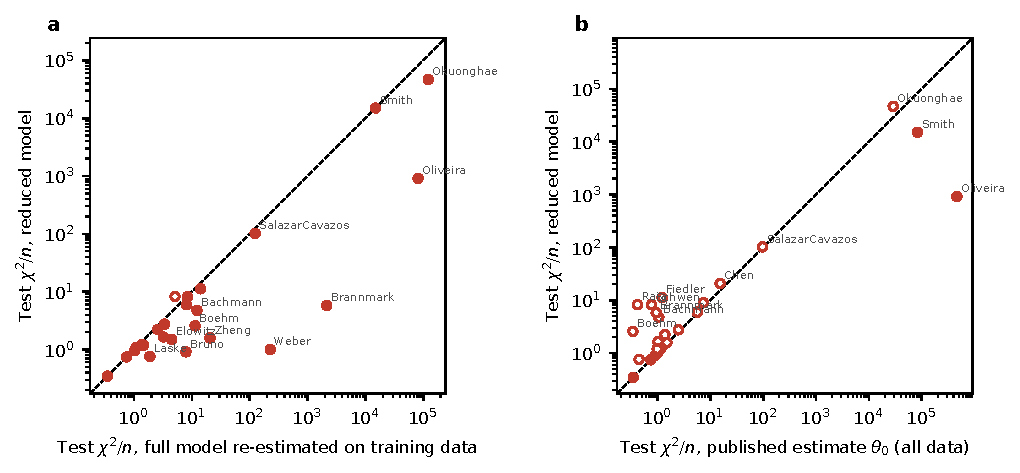
\includegraphics[width=\textwidth,height=0.8\textheight,keepaspectratio]{figures/fig3_validation.pdf}
\caption{\textbf{Prediction of held-out experiments with real data.} Ratio of the test $\chi^2/n$ (mean squared noise-scaled residual on the held-out experiments) of the reduced model to that of a reference, on a logarithmic scale. \textbf{a}, Reference: the full model re-estimated on the same training data ($n=26$ problems). \textbf{b}, Reference: the published estimate $\theta_0$, obtained using all data including the test experiments ($n=27$). Left of the vertical line (circles) the reduced model predicts better; the grey band marks equivalence within 5\% (squares); triangles mark worse predictions. Labels give the ratio; $\blacklozenge$ flags a reduced test $\chi^2/n$ above 10, where a favourable ratio does not imply a good absolute fit. Problems without a training/test split (Bertozzi, Blasi), without a full re-estimation (Lang; \textbf{a} only) or with noise-free data (test $\chi^2/n$ of $\theta_0$ below 0.01: Giordano, Perelson, Rahman) are not shown. Supplementary Fig.~S1 shows the same comparison as a scatter plot (Supplementary Note \textit{Prediction of held-out experiments}).}
\label{fig:validation}
\end{figure}

\begin{table}[p]
\caption{\textbf{External validation against three baseline selectors.} For each of the 28 evaluated problems, test $\chi^2/n$ of our method ($\chi^2_{\mathrm{ours}}$), of calibration-only re-estimation with no biological parameters ($\chi^2_{\mathrm{vac}}$, $|S|=0$), of column-pivoted QR (Brun \emph{et al.}\,\cite{bib9}; $\chi^2_{\mathrm{QR}}$), and of random biological subsets of the same size $k$ (median over 20 independent draws; $\chi^2_{\mathrm{rand}}$). Values near 1 indicate errors comparable to the measurement noise. Category: \textbf{S}, sloppy---all four values within 10\% of each other; \textbf{C}, calibration dominates---re-estimating biological parameters from $\theta_0$ on partial data worsens prediction (bold, lowest value); \textbf{O}, our method clearly best (bold); \textbf{P}, all methods near zero ($<$0.01); \textbf{F}, all methods fail ($\chi^2/n\gg1$). Supplementary Note~\emph{\nt{brun}} gives per-problem parameter lists for the QR comparison (Supplementary Table~S15).}
\label{tab:controls}
\centering
\scriptsize
\setlength{\tabcolsep}{3.5pt}
\renewcommand{\arraystretch}{0.88}
\begin{tabular}{@{}lrccccc@{}}
\toprule
Problem & $k$ & $\chi^2_{\mathrm{ours}}$ & $\chi^2_{\mathrm{vac}}$ & $\chi^2_{\mathrm{QR}}$ & $\chi^2_{\mathrm{rand}}$ & Cat. \\
\midrule
Alkan        & 2  & 2.748 & 2.720 & 2.727 & 2.722 & S \\
Armistead    & 2  & 1.218 & 1.157 & 1.207 & 1.159 & S \\
Bachmann     & 2  & 4.768 & 4.759 & 4.746 & 4.845 & S \\
Boehm        & 2  & 2.567 & \textbf{0.341} & \textbf{0.349} & 1.095 & C \\
Borghans     & 2  & 0.743 & 0.778 & 0.776 & 0.768 & S \\
Brannmark    & 2  & 5.956 & \textbf{0.938} & \textbf{0.951} & 2.952 & C \\
Bruno        & 5  & 0.909 & 0.909 & 0.911 & 0.911 & S \\
Elowitz      & 2  & 1.498 & 1.391 & 1.407 & 1.439 & S \\
Fiedler      & 2  & 11.21 & 11.73 & 10.95 & 11.22 & S \\
Fujita       & 2  & 5.939 & 5.937 & 5.941 & 6.022 & S \\
Giordano     & 2  & $<$0.01 & $<$0.01 & $<$0.01 & $<$0.01 & P \\
Isensee      & 2  & 1.082 & 1.081 & 1.081 & 1.081 & S \\
Laske        & 2  & 0.758 & \textbf{0.445} & \textbf{0.445} & \textbf{0.445} & C \\
Liu          & 2  & 0.954 & 0.942 & 1.026 & 0.942 & S \\
Lucarelli    & 10 & 1.659 & \textbf{1.015} & 1.073 & 1.059 & C \\
Okuonghae    & 2  & $4.7\times10^4$ & $2.9\times10^4$ & $3.2\times10^4$ & $5.6\times10^4$ & F \\
Oliveira     & 2  & \textbf{912} & $4.6\times10^5$ & $7.3\times10^4$ & $2.0\times10^4$ & O \\
Perelson     & 2  & $<$0.01 & $<$0.01 & $<$0.01 & $<$0.01 & P \\
Rahman       & 2  & $<$0.01 & $<$0.01 & $<$0.01 & $<$0.01 & P \\
Raia         & 2  & 8.224 & \textbf{0.439} & 7.236 & 2.213 & C \\
Raimundez    & 2  & 1.188 & 1.167 & 1.168 & 1.181 & S \\
Salazar-C.   & 2  & 101.8 & 96.93 & 101.7 & 103.2 & F \\
Schwen       & 2  & 8.196 & 8.063 & 8.432 & 8.353 & S \\
Smith        & 2  & $1.5\times10^4$ & $1.6\times10^4$ & $1.5\times10^4$ & $1.6\times10^4$ & F \\
Sneyd        & 2  & 2.222 & \textbf{1.373} & 1.480 & 1.890 & C \\
Weber        & 2  & 1.001 & 0.997 & 0.997 & 1.014 & S \\
Zhao         & 3  & 0.345 & 0.345 & 0.345 & 0.345 & P \\
Zheng        & 2  & 1.582 & 1.505 & 1.553 & 1.521 & S \\
\botrule
\end{tabular}
\end{table}

\subsection*{Robustness to the size of parameter changes}\label{sec:patterns}\pdfbookmark[1]{Robustness to the size of parameter changes}{bm7}

Admissibility is decided with perturbations of $\pm$5\%. To determine how far the conclusion extends, we kept each final subset fixed and repeated the evaluation with perturbations of $\pm$1, 5, 10, 20, 30, 40 and 50\% (15 scenarios per level). The scenarios are paired: the same fifteen random directions $u^{(k)}$ are used at every level, $\theta^{(k)}=\theta_0\odot(1+\varepsilon u^{(k)})$, so that differences between levels are due only to the size $\varepsilon$, and the $\pm$5\% level reproduces the scenarios of the selection. We classified the behaviour of the median $e_{\mathrm{fit}}$ into four patterns: A, admissible at all levels; B, admissible up to at least $\pm$20\% and not thereafter; C, irregular (failing and then passing again); D, failing at $\pm$10\% or less.

All 32 admissible problems were evaluated. Twenty-seven follow pattern A (Fig.~\ref{fig:robustness}): their median $e_{\mathrm{fit}}$ stays below the threshold up to $\pm$50\%, typically varying by only a few percentage points across levels. Four follow pattern B: Armistead, whose error grows steadily from 3\% at $\pm$1\% to 63\% at $\pm$50\%, and Bertozzi, Blasi and Elowitz, which are close to the threshold already at $\pm$5\% and cross it between $\pm$20\% and $\pm$30\%. Lucarelli is the only case of pattern C: its median error stays between 43\% and 47\% at all levels, that is, on the threshold rather than clearly above or below it. No problem follows pattern D. The median does not show how many individual scenarios are reproduced, so we also report the pass rate, the fraction of the fifteen scenarios with $e_{\mathrm{fit}}\le\tau_e$ (Fig.~\ref{fig:robustness}b). At $\pm$5\%, 15 of the 32 problems reproduce the full model in all fifteen scenarios and the median pass rate is 93\%; the other 17 have at least one scenario above the threshold. Among the 27 problems of pattern A, 10 pass every scenario at every level, whereas 7 (Borghans, Bruno, Fujita, Liu, Sneyd, Zhao, Zheng) fall to a pass rate of 60--73\% at some level, so their median is below the threshold while four to six of the fifteen scenarios are not reproduced. The reductions therefore remain valid well beyond the $\pm$5\% used for selection in most problems, whereas problems that are admissible only with a small margin at $\pm$5\% are those that lose admissibility for large changes. The full distribution of the error for every problem and level (interquartile range, 5--95\% range, maximum and pass rate) is given in Supplementary Note \textit{Robustness to the size of parameter changes} (Supplementary Tables~S10 and~S11 and Supplementary Fig.~S2).

\begin{figure}[t]
\centering
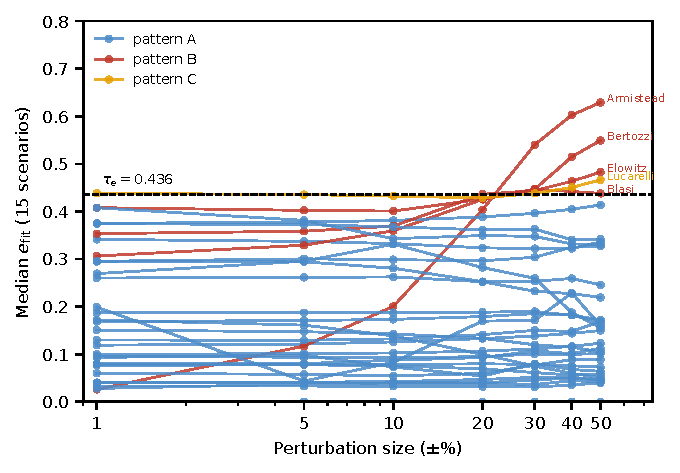
\includegraphics[width=0.66\textwidth]{figures/fig4_robustness.pdf}
\caption{\textbf{Robustness of the selected subsets to the size of parameter changes.} \textbf{a}, Median relative error after re-estimation ($e_{\mathrm{fit}}$) over 15 random scenarios per level as a function of the perturbation size, for the final subset of each of the 32 admissible problems, coloured by robustness pattern (A, admissible at all levels; B, admissible up to at least $\pm$20\%; C, irregular); dashed line, $\tau_e=43.6\%$. \textbf{b}, Pass rate: percentage of the scenarios with $e_{\mathrm{fit}}\le\tau_e$, with the value written when it is below 100\%. The same fifteen random directions are used at every level. --, no valid scenario (Perelson at $\pm$1\%, where the output change is below the numerical noise floor).}
\label{fig:robustness}
\end{figure}

\subsection*{Sensitivity to method settings and computational cost}\label{sec:settings}\pdfbookmark[1]{Sensitivity to method settings and computational cost}{bm8}

The method depends on a finite-difference step $\delta$, integrator tolerances, the perturbation size used for admissibility and four thresholds ($\tau_R$, $\tau_\kappa$, $\tau_{\mathrm{VIF}}$, $\tau_e$). We re-ran the complete method on the 26 small and medium problems changing one setting at a time (Fig.~\ref{fig:settings}). The selected subset was identical to the baseline in all 26 problems for $\delta=0.1\%$ and $5\%$, for both sets of integrator tolerances and for $\tau_R$ between 0.80 and 0.95; with perturbations of $\pm$1\% or $\pm$10\% it differed only in Zhao, where backward elimination removed one of its three parameters, and admissibility changed only for Perelson at $\pm$1\%, where the perturbed output change falls below the numerical noise floor (Supplementary Note \textit{Sensitivity to the method settings}). The $\kappa$/VIF threshold changed the subset in three or four problems without changing the number of admissible problems. As expected, the error threshold $\tau_e$ has the largest influence: requiring $e_{\mathrm{fit}}\le 10\%$ leaves 22 admissible problems with a mean of 3.6 biological parameters, whereas $\tau_e$ between 0.30 and 0.50 gives 25 admissible problems with 2.1--2.4 parameters. The threshold therefore acts as an accuracy--parsimony trade-off that the user can set; we also examined single-parameter subsets: in 16 of the 27 problems examined, a single biological parameter re-estimated together with the calibration parameters reached the threshold at $\pm$5\%, but in the synthetic prediction experiment the selected subset predicted better in 10 of these 16 (Supplementary Note \textit{Single-parameter subsets}, Supplementary Table~S13), which supports the minimum size of two. The value $\tau_e=0.436$ is not a free parameter: it is determined by the cosine requirement $c=0.9$ through $\tau_e=\sqrt{1-c^2}$ (Theorem~\ref{thm:cos}), so the only choice is $c$, whose effect is covered by the $\tau_e$ scan. The admissibility test uses the median over $N=15$ random scenarios rather than requiring all of them to pass, because individual scenarios near the boundary of the parameter domain can fail due to ODE nonlinearity rather than identifiability; for six problems the fraction of passing scenarios is 53--60\% (8--9 of 15), and in all six cases the external test $\chi^2/n$ confirms that the reduced model predicts the held-out data (Supplementary Table~S1). For Lucarelli, the linearised first-order $e_{\mathrm{fit}}$ used for this 84-parameter model gives a median of 0.436, which lies within $5\times10^{-4}$ of $\tau_e$; the external test $\chi^2/n=1.66$ on 598 held-out measurements provides the decisive confirmation of admissibility independent of this borderline criterion. The random seed and the number of scenarios $N$ were not varied in the sensitivity analysis; varying them would only affect problems where not all scenarios pass, and for those six borderline cases the external validation serves as the seed-independent reference.

The dominant cost is the computation of $J$ (2$p$ simulations) and of the stage-2 ordering ($p$ simulations), so the number of simulations grows linearly with the number of parameters, and all of them are independent and can run in parallel; the selection, condition-number tests, backward elimination and the first-order version of $e_{\mathrm{fit}}$ only use linear algebra on $J$. On a four-core server, these simulations took less than 40~s for all but two of the problems we timed, 2~min for Lang (294 parameters) and 68~min for Chen (155 parameters, 35~s per simulation; Supplementary Note \textit{Computational cost}, Supplementary Table~S17). On state trajectories, the 4,231-parameter Froehlich model required 12,693 simulations and 2.6~h. For models of this size on measured outputs, forward or adjoint sensitivity equations\cite{bib13} compute $J$ at the cost of a few simulations.

\begin{figure}[t]
\centering
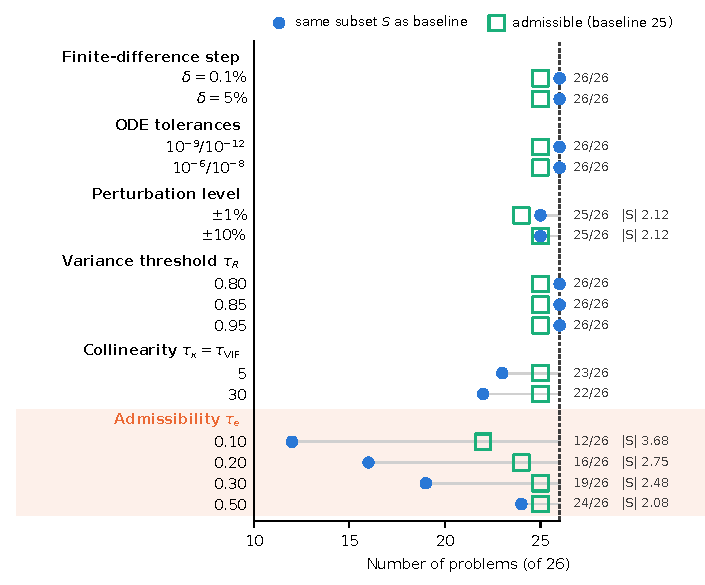
\includegraphics[width=0.66\textwidth]{figures/fig5_settings.pdf}
\caption{\textbf{Sensitivity of the selection to the method settings.} The complete method was re-run on 26 problems changing one setting at a time with respect to the baseline ($\delta=1\%$, tolerances $10^{-7}/10^{-10}$, perturbation $\pm$5\%, $\tau_R=0.89$, $\tau_\kappa=\tau_{\mathrm{VIF}}=10$, $\tau_e=0.436$; 25 admissible problems with a mean of 2.16 selected biological parameters). $\delta$, relative step of the finite differences used for $J$; ODE tolerances, relative/absolute tolerances of the integrator; perturbation level, size of the random parameter changes used for admissibility; $\tau_R$, $\tau_\kappa$, $\tau_{\mathrm{VIF}}$ and $\tau_e$, thresholds on $R_{\mathrm{var}}$, condition number, VIF and $e_{\mathrm{fit}}$. Filled circles, number of problems whose selected subset is identical to the baseline (also given as a fraction on the right); open squares, number of problems with an admissible subset; dashed line, all 26 problems. $|S|$, mean number of selected biological parameters among admissible problems, shown only where it differs from the baseline. The admissibility threshold $\tau_e$ (shaded) is the only setting with a large effect. Results for every problem are given in Supplementary Table~S16.}
\label{fig:settings}
\end{figure}

\subsection*{Formal verification of the mathematical foundations}\label{sec:formal}\pdfbookmark[1]{Formal verification of the mathematical foundations}{bm9}

The mathematical statements on which the method relies and that are verified in Lean~4 with Mathlib are summarised in Supplementary Table~S3; the complete development comprises 31 modules with 289 theorems and lemmas and 28 verified benchmark models; Supplementary Tables~S5 and~S6 give the notation of the formalisation and the statement of every theorem and lemma, and all proofs compile together with a single command (Code availability). None of the proofs uses unproved assumptions (\texttt{sorry}) or additional axioms. Two statements are central to the method:

\begin{theorem}\label{thm:cos}
For vectors $d\neq 0$ and $b\neq 0$ in a real inner-product space, $\min_{\lambda\in\mathbb{R}}\|d-\lambda b\|/\|d\| = \sqrt{1-\cos^2(d,b)}$.
\end{theorem}

\begin{theorem}\label{thm:prune}
Let $\mathcal{A}$ be any admissibility predicate on finite sets and $S$ an admissible set. Backward elimination (removing one element at a time whenever the remaining set is still admissible, until no element can be removed) returns an admissible subset of $S$ from which no element can be removed without losing admissibility.
\end{theorem}

Theorem~\ref{thm:cos} relates the threshold $\tau_e$ to the cosine: whenever $\cos\Delta\ge c$, rescaling the reduced response already gives a relative error of at most $\sqrt{1-c^2}$, and re-estimating several parameters can only do better to first order. The converse does not hold, and admissibility itself is decided by the numerically computed $e_{\mathrm{fit}}$. Theorem~\ref{thm:prune} gives the precise sense in which the selected subsets are minimal: no parameter can be removed, although a different, smaller admissible subset that is not contained in the result may exist. The other verified statements cover the remaining steps: re-estimating more parameters never increases the fitting error and $e_{\mathrm{fit}}\le e_{\mathrm{rel}}$; the selection keeps $\kappa$ and VIF below their thresholds and permanently discarding a rejected candidate is correct because both quantities can only increase when parameters are added; $\kappa$ and VIF bounds imply that the linearised least-squares problem for the retained parameters has a unique and stable solution (which is not a proof of identifiability of the nonlinear model); error bounds on the states transfer to the measured outputs, including logarithmic transformations; and the first-order version of $e_{\mathrm{fit}}$ used for the largest models differs from the exact one by a second-order term. The verification is local: it does not prove that a subset remains adequate far from $\theta_0$, which is assessed empirically above. The theorems are implications; the quantities to which they are applied ($\kappa$, VIF, $R_{\mathrm{var}}$, $e_{\mathrm{fit}}$) are computed in floating point, and Supplementary Table~S4 states the scope of each guarantee and the numerical values that connect it with our results. The model files used by Lean were checked against the SBML models of the benchmark, with agreement to rounding error (Supplementary Note \textit{Verified benchmark models}, Supplementary Table~S7, with the complete data of one model in Supplementary Table~S8). Figure~\ref{fig:architecture} summarises how the two parts fit together: Python performs every computation on the benchmark problems, Lean proves the general statements of Supplementary Table~S3 and checks the hypotheses of each model, and a conclusion of Supplementary Table~S3 applies to a result of the paper only when both the model hypotheses are verified and the computed quantities satisfy the inequalities that the theorem requires.

\begin{figure}[t]
\centering
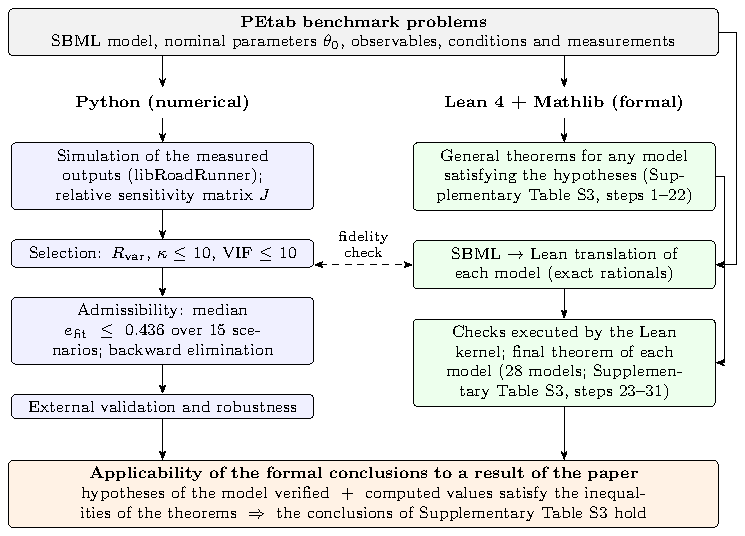
\includegraphics[width=\textwidth]{figures/fig6_architecture.pdf}
\caption{\textbf{Architecture of the formal and numerical verification.} Python (left) performs all computations on the PEtab problems: simulation, sensitivities, selection, admissibility, validation and robustness. Lean~4 with Mathlib (right) proves the general theorems behind each step of the method (Supplementary Table~S3) and, for 28 benchmark models translated from SBML, checks with the Lean kernel that the hypotheses on the dynamics hold. The translation of each model is compared independently with the SBML model (dashed arrow; Supplementary Note \textit{Verified benchmark models}). A formal conclusion applies to a result of the paper when the hypotheses of the model are verified and the numerical quantities computed in Python satisfy the inequalities that the theorem requires (bottom); Supplementary Table~S4 gives, for each guarantee, what it establishes and what it does not.}
\label{fig:architecture}
\end{figure}

\section*{Discussion}\label{sec:discussion}\pdfbookmark[0]{Discussion}{bm10}

The central finding is that, for most published systems biology models with real data, the measured outputs can be reproduced by re-estimating only two biological parameters plus the measurement calibration parameters, and that such reduced models predict held-out experiments as well as or better than the full models. A leakage-free nested validation --- in which the nominal parameter values and optimisation bounds used for the reduced model are derived exclusively from training data --- confirmed that this predictive advantage holds independently of any information that $\theta_0$ carries about the test set: the test $\chi^2/n$ of the nested reduced model matched that of the full model within 1\% in 25 of 28 evaluated problems (within 0.1\% for 19 of the 28). This is consistent with the sloppy-model picture\cite{bib15}, but it is a stronger and more practical statement: it refers to the outputs that were actually measured, under the actual experimental conditions and noise levels, and it is checked by re-estimation and external validation rather than inferred from the sensitivity spectrum alone. The two-stage design reflects a practical observation: ranking by local sensitivity energy (stage~1) was sufficient in only seven problems, whereas ranking by finite-perturbation effects (stage~2) was needed in most. Energy measures how strongly a parameter moves the outputs, not whether adjusting it can compensate for changes in other parameters; the admissibility test, which re-estimates the subset, is what decides.

The method complements existing approaches. Profile likelihood\cite{bib24,bib25} and likelihood-based observability analysis\cite{bib17} assess identifiability after calibration and require repeated optimisation in the full parameter space; profile-likelihood-based model reduction\cite{bib37} identifies parameters to fix but does not validate a re-estimated reduced model on held-out data. Bayesian approaches such as approximate Bayesian computation\cite{bib20} require many more simulations. Global sensitivity analysis\cite{bib26,bib23} and parameter identifiability screening\cite{bib38} rank parameters by importance or linear independence but do not produce a non-redundant subset validated by re-estimation; structural identifiability analysis\cite{bib4,bib10,bib29} addresses ideal noise-free data rather than a given experimental design. Manifold-based sloppiness methods\cite{bib36} identify emergent parameter combinations but do not prescribe which individual parameters to re-estimate. Model-order reduction methods such as balanced truncation\cite{bib22,bib1} reduce the number of state variables rather than parameters. Hierarchical optimisation\cite{bib39} eliminates calibration parameters analytically during fitting but does not select among biological parameters. The collinearity criterion of Brun \emph{et al.}\,\cite{bib9} shares our stage-1 sensitivity ranking but does not include re-estimation, an admissibility check, or backward elimination; the comparison in the Results section shows that both criteria achieve similar external validation accuracy on this benchmark. Our method requires a number of simulations that grows linearly with the number of parameters, is applied before any new calibration, uses published parameter values as its starting point, and returns a concrete subset with documented fidelity, prediction and robustness.

Several limitations should be noted. First, the analysis is local: sensitivities are computed at the published estimate $\theta_0$, which is assumed to be a good fit to the data, and admissibility is tested with perturbations around it. The robustness analysis shows that most reductions remain valid for changes of up to $\pm$50\%, but this cannot be assumed for every model, and problems that are admissible with a small margin at $\pm$5\% (Bertozzi, Blasi, Elowitz, Lucarelli) are those that lose admissibility for larger changes. Second, the method assumes that the model is smooth in the parameters, that the measurement noise is Gaussian with the standard deviations recorded in the benchmark and that the calibration parameters can always be re-estimated; in three problems the recorded noise levels do not match the scatter of the data, and in problems with many calibration parameters (Bachmann, Raimundez) the reduced problem is still sizeable. Third, for the eight problems with the most expensive simulations the fitting error was computed to first order; the verified bounds show that the difference from the exact error is of second order in the perturbation, but it was not quantified numerically for each model. Fourth, one benchmark problem with 9,169 experimental conditions was too expensive to analyse on its measured outputs with finite differences, and two problems had no admissible subset: Beer, and Crauste, whose model has no solution on the measured horizon for parameter changes of 1\%. Finally, the formal verification covers the mathematical steps of the method and the regularity of the translated models, not the numerical simulator itself; we cross-checked our simulations against the reference simulations distributed with the benchmark.

The social cognitive theory model, which motivated this work, illustrates the same behaviour outside molecular biology: with a single measured output the full estimation problem is ill-posed, and the conditioning test identifies two parameters that carry the information in that output, and the reduced model predicts held-out days better than the full one. In practice, the method can be used as a preprocessing step: before calibrating a large model, select the few biological parameters that the data can inform, re-estimate them together with the calibration parameters, keep the rest at literature values, and verify the reduced model on held-out experiments. The threshold $\tau_e$ provides an explicit trade-off between accuracy and parsimony. Natural extensions include computing $J$ with forward or adjoint sensitivity equations for genome-scale models, combining sensitivities at several operating points, and using the selected subsets to guide experimental design\cite{bib28}.

\section*{Methods}\label{sec:methods}\pdfbookmark[0]{Methods}{bm11}

\subsection*{Models, data and simulation}\pdfbookmark[1]{Models, data and simulation}{bm12}

We used the problems of the PEtab benchmark collection\cite{bib31,bib27} that provide real measurements, an SBML model and nominal parameter values (34 problems; Table~\ref{tab:benchmark}). Each problem specifies the observables $g_i$, their transformation $h$ (linear, $\log$ or $\log_{10}$), the noise standard deviation $\sigma_i$ of each measurement, the experimental conditions (parameter or initial-value overrides) and, where applicable, pre-equilibration conditions. Models were simulated with libRoadRunner\cite{bib32} (CVODE, relative and absolute tolerances $10^{-7}$ and $10^{-10}$). Initial assignments that depend on parameters were re-evaluated for every parameter vector, condition-specific overrides were applied before simulation, pre-equilibration was run to steady state before the main simulation, and models with discontinuous inputs were integrated piecewise between discontinuities. Simulated observables were compared with the reference simulations distributed with the benchmark wherever available (Supplementary Note \textit{Verification of the simulator}, Supplementary Table~S9).

\subsection*{Social cognitive theory model}\pdfbookmark[1]{Social cognitive theory model}{bm13}

The model\cite{bib34,bib35} has six states $x_i$ (constructs of social cognitive theory\cite{bib3}) and obeys $\dot x=A(\theta)x+B(\theta)u$, $y=x_4$ (behaviour), with $A_{ii}=-1/\tau_i$, $A_{ij}=\beta_{ij}/\tau_i$ for the ten couplings $\beta_{14},\beta_{21},\beta_{25},\beta_{31},\beta_{34},\beta_{42},\beta_{43},\beta_{45},\beta_{46},\beta_{54}$, and input gains $\gamma_{33},\gamma_{35},\gamma_{36},\gamma_{57},\gamma_{64},\gamma_{68}$ divided by the time constant of the receiving construct ($\gamma_{35}$ enters with negative sign; 22 parameters). The data are 31 daily records of one participant\cite{bib35}: six measured inputs and daily steps as output, each standardised to zero mean and unit variance. The model is simulated from $x(0)=0$ with inputs held constant over each day (exact zero-order-hold discretisation with the matrix exponential), and the output of day $k$ is $x_4$ at the end of that day. $\theta_0$ minimises the mean squared error by differential evolution, following the estimation framework of ref.~\cite{bib35} (strategy best1bin, population factor 4, 60 generations, Latin hypercube initialisation, no polishing; 5,368 function evaluations; seed 2026) within the bounds $\beta\in[-1.5,1.5]$, $\gamma\in[0,3]$, $\tau\in[0.3,12]$, subject to stability ($\max\operatorname{Re}\lambda(A)\le-10^{-3}$); the 100 runs with seeds 2026--2125 were used only to assess non-identifiability. The noise level $\sigma$ is the standard deviation of the residuals at $\theta_0$ (0.35 in standardised units). Because couplings may be negative, the reduced refit uses $\theta_j=\operatorname{sign}(\theta_{0,j})\exp(v_j)$. All other settings are as for the benchmark problems. For validation, the reduced and full models were refitted to days 1--24 by least squares from $\theta_0$ within the same bounds and with the stability constraint, and the full model also by the same differential-evolution search; both were evaluated on days 25--31.

\subsection*{Measured outputs and parameter classes}\pdfbookmark[1]{Measured outputs and parameter classes}{bm14}

For a parameter vector $\theta\in\mathbb{R}^p$ (in the units of the benchmark, excluding noise parameters), the vector of scaled outputs is $y(\theta)\in\mathbb{R}^m$ with entries
\begin{equation}
y_i(\theta)=\frac{h\big(g_i(x(t_i;\theta,c_i),\theta)\big)}{\sigma_i},\qquad i=1,\dots,m,
\label{eq:outputs}
\end{equation}
where $x(t;\theta,c)$ is the state trajectory under condition $c$ and $(t_i,c_i)$ are the time and condition of measurement $i$. Parameters that appear in the SBML model are biological ($\Theta_B$); parameters that appear only in the observation functions and not in the model or the condition table (scalings and offsets) are calibration parameters ($\Theta_C$). Only biological parameters are candidates for selection; calibration parameters are always re-estimated.

\subsection*{Sensitivities, energy and conditioning}\pdfbookmark[1]{Sensitivities, energy and conditioning}{bm15}

The relative sensitivity matrix $J\in\mathbb{R}^{m\times p}$ is computed by central differences,
\begin{equation}
J_{:,j}=\frac{y(\theta_0+\delta\theta_{0,j}e_j)-y(\theta_0-\delta\theta_{0,j}e_j)}{2\delta},
\label{eq:jac}
\end{equation}
which approximates $\partial y/\partial\log\theta_j$. The energy of parameter $j$ is $E_j=\|J_{:,j}\|^2=(J^\top J)_{jj}$ and the fraction of energy captured by a subset $S\subseteq\Theta_B$ is $R_{\mathrm{var}}(S)=\sum_{j\in S}E_j/\sum_{j\in\Theta_B}E_j$. For a subset $S$, the columns of $J_S$ are normalised to unit length, $Z=J_S\,\mathrm{diag}(\|J_{:,j}\|)^{-1}$; the condition number is $\kappa(S)=\sigma_{\max}(Z)/\sigma_{\min}(Z)$ and the largest variance inflation factor is $\mathrm{VIF}(S)=\max_j[(Z^\top Z)^{-1}]_{jj}$\cite{bib5,bib9}. Normalisation removes differences of scale between parameters, so that $\kappa$ and VIF measure only the angles between sensitivity directions.

\subsection*{Selection}\pdfbookmark[1]{Selection}{bm16}

\emph{Greedy selection.} Candidates are visited in a given order. A candidate $j$ is accepted if $\kappa(S\cup\{j\})\le\tau_\kappa$ and $\mathrm{VIF}(S\cup\{j\})\le\tau_{\mathrm{VIF}}$; otherwise it is discarded permanently. Because $\kappa$ and VIF can only increase when columns are added, a discarded candidate would also be rejected later. \emph{Stage~1} visits biological parameters in decreasing order of $E_j$ and stops when $R_{\mathrm{var}}(S)\ge\tau_R$. \emph{Stage~2}, used if the stage-1 subset is not admissible, visits biological parameters in decreasing order of the finite-perturbation effect $s_j=\|y(\theta_0+\eta\theta_{0,j}e_j)-y(\theta_0)\|$ and stops at the first admissible subset. \emph{Backward elimination} visits the parameters of the selected subset and removes each one whose removal leaves the subset admissible.

\subsection*{Admissibility and re-estimation}\pdfbookmark[1]{Admissibility and re-estimation}{bm17}

Admissibility is evaluated on $N$ random scenarios $\theta^{(k)}=\theta_0\odot(1+\varepsilon u^{(k)})$, with $u^{(k)}$ uniform in $[-1,1]^p$. For each scenario let $\Delta y_{\mathrm{full}}=y(\theta^{(k)})-y(\theta_0)$. The relative error without re-estimation is $e_{\mathrm{rel}}=\|\Delta y_{\mathrm{full}}-\Delta y_S\|/\|\Delta y_{\mathrm{full}}\|$, where $\Delta y_S$ is the output change when only the parameters in $S\cup\Theta_C$ take their scenario values, and the cosine similarity is $\cos\Delta=\langle\Delta y_{\mathrm{full}},\Delta y_S\rangle/(\|\Delta y_{\mathrm{full}}\|\|\Delta y_S\|)$. The relative error after re-estimation is
\begin{equation}
e_{\mathrm{fit}}=\min_{\theta_{S},\theta_C}\frac{\|y(\theta_S,\theta_C,\theta_{0,\overline{S}})-y(\theta^{(k)})\|}{\|\Delta y_{\mathrm{full}}\|},
\label{eq:efit}
\end{equation}
where $\theta_{0,\overline{S}}$ denotes the nominal values of all other biological parameters. The minimisation is carried out in $\log|\theta|$ within $[|\theta_0|/10,\,10|\theta_0|]$ by a trust-region reflective least-squares method (SciPy\cite{bib33}, at most $100(|S|+|\Theta_C|+1)$ function evaluations), from two starting points (the scenario value and $\theta_0$); the error without re-estimation is also included, so that $e_{\mathrm{fit}}\le e_{\mathrm{rel}}$. Scenarios whose output change is below $\max(10^{-10}\|y(\theta_0)\|,10^{-6})$ are discarded. $S$ is admissible if $|S|\ge k_{\min}$ and the median of $e_{\mathrm{fit}}$ over the scenarios is at most $\tau_e=\sqrt{1-c^2}$. For each admissible subset we also report a level of guarantee: level~1 when only this condition holds, level~2 when in addition the median $\cos\Delta$ is at least $c$, and level~3 when in addition $R_{\mathrm{var}}(S)\ge\tau_R$; these levels are reported, not required. For the eight problems in which the cost of simulation made repeated re-estimation impractical (marked in Table~\ref{tab:benchmark}), the first-order version $\min_c\|\Delta y_{\mathrm{full}}-J_{S\cup\Theta_C}c\|/\|\Delta y_{\mathrm{full}}\|$ was used. This equals the minimum relative error attainable if the model response were exactly linear in parameter changes; for a truly linear model it equals the exact $e_{\mathrm{fit}}$, while for nonlinear models it is an approximation (exact to second order) that replaces per-scenario optimisation with a single projection. The admissibility decision for these eight models is therefore made on linear-algebra alone; the external test $\chi^2/n$ on held-out data provides independent confirmation of practical admissibility for all eight.

\subsection*{Settings}\pdfbookmark[1]{Settings}{bm18}

Unless stated otherwise: $\delta=0.01$; $\eta=0.1$; $\tau_R=0.89$; $\tau_\kappa=\tau_{\mathrm{VIF}}=10$; $N=15$ scenarios; $\varepsilon=0.05$; random seed 42; $c=0.9$, so $\tau_e=0.436$; $k_{\min}=2$. The sensitivity analysis (Fig.~\ref{fig:settings}) changed one setting at a time on the 26 problems that could be re-run completely in reasonable time.

\subsection*{External validation}\pdfbookmark[1]{External validation}{bm19}

Measurements were split into training and test sets by experimental condition (every third condition after sorting, or the second of two conditions, used for testing) or, for problems with a single condition, by time (the last third of the distinct measurement times). Parameters that only affect test conditions were excluded from re-estimation. The reduced model (re-estimating $S\cup\Theta_C$) and the full model (re-estimating all parameters; not done for Lang, with 277 parameters and slow simulations, because it would require days to weeks of computation) were fitted to the training data from $\theta_0$ with the same least-squares method and bounds, and evaluated by the mean squared noise-scaled residual $\chi^2/n=\frac{1}{n}\sum_{i\in\mathrm{test}}(y_i(\hat\theta)-\tilde y_i)^2$, where $\tilde y_i$ are the scaled measurements. In the synthetic experiment, the truth $\theta^\ast$ had each parameter drawn uniformly within $\pm$20\% of $\theta_0$, data were simulated with Gaussian noise of standard deviation $\sigma_i$, and $e_{\mathrm{pred}}=\|y_{\mathrm{test}}(\hat\theta)-y_{\mathrm{test}}(\theta^\ast)\|/\|y_{\mathrm{test}}(\theta^\ast)-y_{\mathrm{test}}(\theta_0)\|$; the effect of the parameter change was considered larger than the noise when $\chi^2/n$ of $\theta_0$ on the synthetic test data was at least 2. Problems whose test $\chi^2/n$ at $\theta_0$ was below 0.01 (Giordano, Perelson, Rahman) reproduce the data to far below the recorded noise level; their $\chi^2/n$ values are not comparable and they are counted in the text but not shown in Fig.~\ref{fig:validation}. Test errors were compared through the ratio of the reduced to the reference $\chi^2/n$; ratios between 0.95 and 1.05 were considered equivalent. For the leakage-free nested validation (Supplementary Note~\textit{Leakage-free nested validation}), the full model was re-estimated on training data first (yielding $\hat\theta_{\mathrm{train}}$), and the reduced model was re-estimated starting from $\hat\theta_{\mathrm{train}}$ with non-selected parameters fixed at $\hat\theta_{\mathrm{train}}$; this required a second optimisation pass per problem and was applied to 28 problems; three admissible problems were excluded (Bertozzi: selected parameters active only in test conditions; Blasi: single time point with no valid split; Lang: 277 parameters, computationally infeasible), and Chen did not complete within the available computation time. The search bounds for the free parameters in the nested optimisation were also derived from $\hat\theta_{\mathrm{train}}$, ensuring no test-set information enters through the optimisation bounds.

\subsection*{Robustness patterns}\pdfbookmark[1]{Robustness patterns}{bm20}

For each admissible problem, the final subset was kept fixed and $e_{\mathrm{fit}}$ was evaluated at perturbation sizes $\varepsilon\in\{0.01,0.05,0.10,0.20,0.30,0.40,0.50\}$ with 15 scenarios per level. The fifteen directions $u^{(k)}\in[-1,1]^p$, with independent uniform components, are drawn once per problem with a fixed seed (42) and reused at every level, $\theta^{(k)}=\theta_0\odot(1+\varepsilon u^{(k)})$; the directions are stored with the results. Patterns were assigned from the median $e_{\mathrm{fit}}$ at each level as described in Results; the pass rate is the fraction of valid scenarios with $e_{\mathrm{fit}}\le\tau_e$. As in the selection, $e_{\mathrm{fit}}$ was computed to first order for the problems marked in Table~\ref{tab:benchmark}. For Chen, between 8 and 13 of the 15 scenarios per level could be simulated; the remaining scenarios failed to integrate and were discarded.

\subsection*{Formal verification}\pdfbookmark[1]{Formal verification}{bm21}

The formal development uses Lean~4 (version 4.23.0) and Mathlib\cite{bib19,bib21} and has two parts (Fig.~\ref{fig:architecture}). The first proves, for any model that satisfies stated hypotheses, the mathematical results on which each step of the method relies (Supplementary Table~S3, steps 1--22). The second establishes those hypotheses for concrete benchmark models. For this, each PEtab problem was translated automatically into a Lean file (\texttt{lean\_translation/sbml\_to\_lean.py} of the reproducibility package): the rate laws and stoichiometry of the SBML model and the nominal parameter values and initial conditions of the PEtab tables are written as Lean expressions in which every number is an exact rational. Verified checkers, Boolean functions proved sound in Lean, then test that every rate law is defined and smooth on a domain containing the trajectory, that concentrations cannot become negative (quasi-positivity) and that the growth of the vector field is bounded so that the solution exists on the simulated horizon (linear growth, or a Riccati bound on a finite horizon for Crauste). The checkers are evaluated by the Lean kernel itself (\texttt{decide +kernel}), so their results are part of the proof, and each model ends with a theorem stating that it is smooth, that its solution exists and remains non-negative on the horizon, and that the solution is differentiable with respect to the parameters, which are the hypotheses of steps 14--22. This was achieved for 28 benchmark models (27 of the 34 problems analysed, and Froehlich); the reasons why the other seven problems were not verified are given in Supplementary Note \textit{Verified benchmark models}. Because the theorems are only as relevant as the translation is faithful, the translated vector fields, parameter values and initial values were compared independently with the SBML models evaluated by libRoadRunner at the nominal state and at five random states; they agree to rounding error (largest relative difference $10^{-12}$), and changing a single number of a Lean file by 1\% is detected. All files compile without \texttt{sorry}, and \texttt{\#print axioms} reports only the standard axioms of Lean's logic (\texttt{propext}, \texttt{Classical.choice}, \texttt{Quot.sound}). The numerical analyses of this paper ($J$, $R_{\mathrm{var}}$, $\kappa$, VIF, $\cos\Delta$, $e_{\mathrm{fit}}$ and the validation) were carried out in Python in double precision; a formal conclusion applies to a numerical result when the model's hypotheses are verified in Lean and the computed quantities satisfy the inequalities that the corresponding theorem requires (Supplementary Table~S4).

\subsection*{Use of large language models}\pdfbookmark[1]{Use of large language models}{bm22}

An AI assistant (Claude, Anthropic) was used to help write and debug analysis code and Lean proofs and to edit the manuscript text. All code, proofs and results were checked by the authors, who take full responsibility for the content.

\backmatter

\bmhead{Data availability}
The PEtab benchmark problems analysed in this study are publicly available in the Benchmark-Models-PEtab collection (\url{https://github.com/Benchmarking-Initiative/Benchmark-Models-PEtab}, commit \texttt{fcbddf1}). All results generated in this study (selected subsets, external validation, robustness, single-parameter subsets, sensitivity to the method settings, simulator check, cost and the checks of the Lean models), one file per benchmark problem with a data dictionary, are included in the reproducibility package archived on Zenodo (\href{https://doi.org/\zenododoi}{doi:\zenododoi}) and in the folder \texttt{reproducibility/} of \url{https://github.com/monicammr/archivos}. The participant's step-count data of the social cognitive theory model are available from the corresponding author on reasonable request.

\bmhead{Code availability}
The reproducibility package (Zenodo, \href{https://doi.org/\zenododoi}{doi:\zenododoi}; folder \texttt{reproducibility/} of \url{https://github.com/monicammr/archivos}) contains the Python code of the method and of every analysis, the programs that produce every figure and table of the paper from the stored results, the translator of the SBML models into Lean, and all Lean~4 proofs (folder \texttt{lean\_proofs/}, a self-contained project that compiles with a single command, \texttt{./verify.sh}, and checks that no proof uses \texttt{sorry} or additional axioms). Its manual (\texttt{README.md}) describes three levels of checking: regenerating the figures and tables from the stored results, compiling the proofs, and re-running the analyses from the PEtab problems; Supplementary Note \textit{Reproducibility package} summarises them.

\bmhead{Acknowledgements}
The authors thank Escuela Superior Polit\'ecnica del Litoral (ESPOL) for institutional support.

\bmhead{Author contributions}
M.M.R. and C.S. conceived the study and designed the method. M.M.R. wrote the software and the formal proofs, performed the analyses and wrote the first draft. C.S., C.M. and A.A. supervised the work, contributed to the validation of the results and revised the manuscript. All authors reviewed and approved the final manuscript.

\bmhead{Funding}
This research received no external funding.

\bmhead{Ethics declarations}
\textbf{Ethics approval and consent to participate:} The step-count data used for the social cognitive theory model were collected in a previously published study\cite{bib35} approved by the Institutional Review Board of that study. The participant provided written informed consent for the use of their anonymised data in subsequent analyses.\\
\textbf{Consent for publication:} The participant whose data underlie the social cognitive theory analysis gave consent for publication of anonymised results.

\bmhead{Additional information}
\textbf{Competing interests:} The authors declare no competing interests.\\
\textbf{Correspondence} and requests for materials should be addressed to M.M.R.\\
\textbf{Supplementary information} accompanies this paper (Supplementary Notes, Supplementary Tables S1--S18 and Supplementary Figs.~S1--S5); Supplementary Note \textit{Concluding remarks} summarises its contents.

\begin{thebibliography}{48}
\expandafter\ifx\csname url\endcsname\relax
  \def\url#1{\burl{#1}}\fi
\expandafter\ifx\csname urlprefix\endcsname\relax\def\urlprefix{URL }\fi
\providecommand{\bibinfo}[2]{#2}
\providecommand{\eprint}[2][]{\url{#2}}
\providecommand{\doi}[1]{\url{https://doi.org/#1}}
\bibcommenthead

\bibitem{bib16}
\bibinfo{author}{Kholodenko, B.~N.}
\newblock \bibinfo{title}{Cell-signalling dynamics in time and space}.
\newblock \emph{\bibinfo{journal}{Nature Reviews Molecular Cell Biology}}
  \textbf{\bibinfo{volume}{7}}, \bibinfo{pages}{165--176}
  (\bibinfo{year}{2006}).

\bibitem{bib4}
\bibinfo{author}{Bellman, R.} \& \bibinfo{author}{{\AA}str{\"o}m, K.~J.}
\newblock \bibinfo{title}{On structural identifiability}.
\newblock \emph{\bibinfo{journal}{Mathematical Biosciences}}
  \textbf{\bibinfo{volume}{7}}, \bibinfo{pages}{329--339}
  (\bibinfo{year}{1970}).

\bibitem{bib10}
\bibinfo{author}{Chi{\c{s}}, O.-T.}, \bibinfo{author}{Banga, J.~R.} \&
  \bibinfo{author}{Balsa-Canto, E.}
\newblock \bibinfo{title}{Structural identifiability of systems biology models:
  A critical comparison of methods}.
\newblock \emph{\bibinfo{journal}{PLOS ONE}} \textbf{\bibinfo{volume}{6}},
  \bibinfo{pages}{e27755} (\bibinfo{year}{2011}).

\bibitem{bib29}
\bibinfo{author}{Villaverde, A.~F.}, \bibinfo{author}{Barreiro, A.} \&
  \bibinfo{author}{Papachristodoulou, A.}
\newblock \bibinfo{title}{Structural identifiability of dynamic systems biology
  models}.
\newblock \emph{\bibinfo{journal}{PLOS Computational Biology}}
  \textbf{\bibinfo{volume}{12}}, \bibinfo{pages}{e1005153}
  (\bibinfo{year}{2016}).

\bibitem{bib49}
\bibinfo{author}{Miao, H.}, \bibinfo{author}{Xia, X.}, \bibinfo{author}{Perelson, A.~S.} \& \bibinfo{author}{Wu, H.}
\newblock \bibinfo{title}{On identifiability of nonlinear {ODE} models and applications in viral dynamics}.
\newblock \emph{\bibinfo{journal}{SIAM Rev.}} \textbf{\bibinfo{volume}{53}}, \bibinfo{pages}{3--39} (\bibinfo{year}{2011}).

\bibitem{bib50}
\bibinfo{author}{Wieland, F.-G.}, \bibinfo{author}{Hauber, A.~L.}, \bibinfo{author}{Rosenblatt, M.}, \bibinfo{author}{T{\"o}nsing, C.} \& \bibinfo{author}{Timmer, J.}
\newblock \bibinfo{title}{On structural and practical identifiability}.
\newblock \emph{\bibinfo{journal}{Curr. Opin. Syst. Biol.}} \textbf{\bibinfo{volume}{25}}, \bibinfo{pages}{60--69} (\bibinfo{year}{2021}).

\bibitem{bib24}
\bibinfo{author}{Raue, A.} \emph{et~al.}
\newblock \bibinfo{title}{Structural and practical identifiability analysis of
  partially observed dynamical models by exploiting the profile likelihood}.
\newblock \emph{\bibinfo{journal}{Bioinformatics}}
  \textbf{\bibinfo{volume}{25}}, \bibinfo{pages}{1923--1929}
  (\bibinfo{year}{2009}).

\bibitem{bib25}
\bibinfo{author}{Raue, A.}, \bibinfo{author}{Kreutz, C.},
  \bibinfo{author}{Theis, F.~J.} \& \bibinfo{author}{Timmer, J.}
\newblock \bibinfo{title}{Joining forces of {Bayesian} and frequentist
  methodology: A study for inference in the presence of non-identifiability}.
\newblock \emph{\bibinfo{journal}{Philosophical Transactions of the Royal
  Society A}} \textbf{\bibinfo{volume}{371}}, \bibinfo{pages}{20110544}
  (\bibinfo{year}{2013}).

\bibitem{bib17}
\bibinfo{author}{Kreutz, C.}, \bibinfo{author}{Raue, A.} \&
  \bibinfo{author}{Timmer, J.}
\newblock \bibinfo{title}{Likelihood based observability analysis and
  confidence intervals for predictions of dynamic models}.
\newblock \emph{\bibinfo{journal}{BMC Systems Biology}}
  \textbf{\bibinfo{volume}{6}}, \bibinfo{pages}{120} (\bibinfo{year}{2012}).

\bibitem{bib31}
\bibinfo{author}{Hass, H.} \emph{et~al.}
\newblock \bibinfo{title}{Benchmark problems for dynamic modeling of intracellular processes}.
\newblock \emph{\bibinfo{journal}{Bioinformatics}} \textbf{\bibinfo{volume}{35}}, \bibinfo{pages}{3073--3082} (\bibinfo{year}{2019}).

\bibitem{bib15}
\bibinfo{author}{Gutenkunst, R.~N.} \emph{et~al.}
\newblock \bibinfo{title}{Universally sloppy parameter sensitivities in systems
  biology models}.
\newblock \emph{\bibinfo{journal}{PLOS Computational Biology}}
  \textbf{\bibinfo{volume}{3}}, \bibinfo{pages}{e189} (\bibinfo{year}{2007}).

\bibitem{bib41}
\bibinfo{author}{Transtrum, M.~K.} \emph{et~al.}
\newblock \bibinfo{title}{Perspective: Sloppiness and emergent theories in physics, biology, and beyond}.
\newblock \emph{\bibinfo{journal}{J. Chem. Phys.}} \textbf{\bibinfo{volume}{143}}, \bibinfo{pages}{010901} (\bibinfo{year}{2015}).

\bibitem{bib53}
\bibinfo{author}{Monsalve-Bravo, G.~M.} \emph{et~al.}
\newblock \bibinfo{title}{Analysis of sloppiness in model simulations: Unveiling parameter uncertainty when mathematical models are fitted to data}.
\newblock \emph{\bibinfo{journal}{Sci. Adv.}} \textbf{\bibinfo{volume}{8}}, \bibinfo{pages}{eabm5952} (\bibinfo{year}{2022}).

\bibitem{bib26}
\bibinfo{author}{Saltelli, A.}, \bibinfo{author}{Tarantola, S.},
  \bibinfo{author}{Campolongo, F.} \& \bibinfo{author}{Ratto, M.}
\newblock \emph{\bibinfo{title}{Sensitivity analysis in practice: A guide to
  assessing scientific models}}  (\bibinfo{publisher}{Wiley},
  \bibinfo{year}{2004}).

\bibitem{bib23}
\bibinfo{author}{Morris, M.~D.}
\newblock \bibinfo{title}{Factorial sampling plans for preliminary
  computational experiments}.
\newblock \emph{\bibinfo{journal}{Technometrics}}
  \textbf{\bibinfo{volume}{33}}, \bibinfo{pages}{161--174}
  (\bibinfo{year}{1991}).

\bibitem{bib37}
\bibinfo{author}{Maiwald, T.} \emph{et~al.}
\newblock \bibinfo{title}{Driving the model to its limit: Profile likelihood
  based model reduction}.
\newblock \emph{\bibinfo{journal}{PLOS ONE}} \textbf{\bibinfo{volume}{11}},
  \bibinfo{pages}{e0162366} (\bibinfo{year}{2016}).

\bibitem{bib51}
\bibinfo{author}{Eisenberg, M.~C.} \& \bibinfo{author}{Hayashi, M.~A.~L.}
\newblock \bibinfo{title}{Determining identifiable parameter combinations using subset profiling}.
\newblock \emph{\bibinfo{journal}{Math. Biosci.}} \textbf{\bibinfo{volume}{256}}, \bibinfo{pages}{116--126} (\bibinfo{year}{2014}).

\bibitem{bib5}
\bibinfo{author}{Belsley, D.~A.}, \bibinfo{author}{Kuh, E.} \&
  \bibinfo{author}{Welsch, R.~E.}
\newblock \emph{\bibinfo{title}{Regression diagnostics: Identifying influential
  data and sources of collinearity}}  (\bibinfo{publisher}{Wiley},
  \bibinfo{year}{1980}).

\bibitem{bib42}
\bibinfo{author}{Weijers, S.~R.} \& \bibinfo{author}{Vanrolleghem, P.~A.}
\newblock \bibinfo{title}{A procedure for selecting best identifiable parameters in calibrating activated sludge model no. 1 to full-scale plant data}.
\newblock \emph{\bibinfo{journal}{Water Sci. Technol.}} \textbf{\bibinfo{volume}{36}}, \bibinfo{pages}{69--79} (\bibinfo{year}{1997}).

\bibitem{bib46}
\bibinfo{author}{Cintr{\'o}n-Arias, A.}, \bibinfo{author}{Banks, H.~T.}, \bibinfo{author}{Capaldi, A.} \& \bibinfo{author}{Lloyd, A.~L.}
\newblock \bibinfo{title}{A sensitivity matrix based methodology for inverse problem formulation}.
\newblock \emph{\bibinfo{journal}{J. Inverse Ill-Posed Probl.}} \textbf{\bibinfo{volume}{17}}, \bibinfo{pages}{545--564} (\bibinfo{year}{2009}).

\bibitem{bib9}
\bibinfo{author}{Brun, R.}, \bibinfo{author}{Reichert, P.} \&
  \bibinfo{author}{K{\"u}nsch, H.~R.}
\newblock \bibinfo{title}{Practical identifiability analysis of large
  environmental simulation models}.
\newblock \emph{\bibinfo{journal}{Water Resources Research}}
  \textbf{\bibinfo{volume}{37}}, \bibinfo{pages}{1015--1030}
  (\bibinfo{year}{2001}).

\bibitem{bib38}
\bibinfo{author}{G{\'a}bor, A.}, \bibinfo{author}{Villaverde, A.~F.} \&
  \bibinfo{author}{Banga, J.~R.}
\newblock \bibinfo{title}{Parameter identifiability analysis and visualization
  in large-scale kinetic models of biosystems}.
\newblock \emph{\bibinfo{journal}{BMC Systems Biology}}
  \textbf{\bibinfo{volume}{11}}, \bibinfo{pages}{54} (\bibinfo{year}{2017}).

\bibitem{bib43}
\bibinfo{author}{Yao, K.~Z.}, \bibinfo{author}{Shaw, B.~M.}, \bibinfo{author}{Kou, B.}, \bibinfo{author}{McAuley, K.~B.} \& \bibinfo{author}{Bacon, D.~W.}
\newblock \bibinfo{title}{Modeling ethylene/butene copolymerization with multi-site catalysts: Parameter estimability and experimental design}.
\newblock \emph{\bibinfo{journal}{Polym. React. Eng.}} \textbf{\bibinfo{volume}{11}}, \bibinfo{pages}{563--588} (\bibinfo{year}{2003}).

\bibitem{bib44}
\bibinfo{author}{Li, R.}, \bibinfo{author}{Henson, M.~A.} \& \bibinfo{author}{Kurtz, M.~J.}
\newblock \bibinfo{title}{Selection of model parameters for off-line parameter estimation}.
\newblock \emph{\bibinfo{journal}{IEEE Trans. Control Syst. Technol.}} \textbf{\bibinfo{volume}{12}}, \bibinfo{pages}{402--412} (\bibinfo{year}{2004}).

\bibitem{bib45}
\bibinfo{author}{Lund, B.~F.} \& \bibinfo{author}{Foss, B.~A.}
\newblock \bibinfo{title}{Parameter ranking by orthogonalization---Applied to nonlinear mechanistic models}.
\newblock \emph{\bibinfo{journal}{Automatica}} \textbf{\bibinfo{volume}{44}}, \bibinfo{pages}{278--281} (\bibinfo{year}{2008}).

\bibitem{bib47}
\bibinfo{author}{Quaiser, T.} \& \bibinfo{author}{M{\"o}nnigmann, M.}
\newblock \bibinfo{title}{Systematic identifiability testing for unambiguous mechanistic modeling -- application to {JAK-STAT}, {MAP} kinase, and {NF-$\kappa$B} signaling pathway models}.
\newblock \emph{\bibinfo{journal}{BMC Syst. Biol.}} \textbf{\bibinfo{volume}{3}}, \bibinfo{pages}{50} (\bibinfo{year}{2009}).

\bibitem{bib40}
\bibinfo{author}{V{\'e}lez-Reyes, M.} \& \bibinfo{author}{Verghese, G.~C.}
\newblock \bibinfo{title}{Subset selection in identification, and application to speed and parameter estimation for induction machines}.
\newblock In \emph{\bibinfo{booktitle}{Proceedings of the 4th IEEE Conference on Control Applications}}, \bibinfo{pages}{991--997} (\bibinfo{year}{1995}).

\bibitem{bib54}
\bibinfo{author}{Golub, G.~H.} \& \bibinfo{author}{Van~Loan, C.~F.}
\newblock \emph{\bibinfo{title}{Matrix Computations}} (\bibinfo{edition}{4th edn}, \bibinfo{publisher}{Johns Hopkins University Press}, \bibinfo{year}{2013}).

\bibitem{bib48}
\bibinfo{author}{Olufsen, M.~S.} \& \bibinfo{author}{Ottesen, J.~T.}
\newblock \bibinfo{title}{A practical approach to parameter estimation applied to model predicting heart rate regulation}.
\newblock \emph{\bibinfo{journal}{J. Math. Biol.}} \textbf{\bibinfo{volume}{67}}, \bibinfo{pages}{39--68} (\bibinfo{year}{2013}).

\bibitem{bib3}
\bibinfo{author}{Bandura, A.}
\newblock \emph{\bibinfo{title}{Social Foundations of Thought and Action: A
  Social Cognitive Theory}}  (\bibinfo{publisher}{Prentice-Hall},
  \bibinfo{year}{1986}).

\bibitem{bib55}
\bibinfo{author}{Mart\'in, C.~A.} \emph{et~al.}
\newblock \bibinfo{title}{A dynamical systems model of social cognitive theory}.
\newblock In \emph{\bibinfo{booktitle}{2014 American Control Conference (ACC)}}, \bibinfo{pages}{2407--2412} (\bibinfo{publisher}{IEEE}, \bibinfo{year}{2014}).

\bibitem{bib56}
\bibinfo{author}{Riley, W.~T.} \emph{et~al.}
\newblock \bibinfo{title}{Development of a dynamic computational model of social cognitive theory}.
\newblock \emph{\bibinfo{journal}{Transl. Behav. Med.}} \textbf{\bibinfo{volume}{6}}, \bibinfo{pages}{483--495} (\bibinfo{year}{2016}).

\bibitem{bib34}
\bibinfo{author}{Mart\'in, C.~A.}, \bibinfo{author}{Rivera, D.~E.}, \bibinfo{author}{Aguirre, A.~A.} \& \bibinfo{author}{Salazar, C.~A.}
\newblock \bibinfo{title}{Dynamic modeling of social cognitive theory constructs in physical activity interventions}.
\newblock \emph{\bibinfo{journal}{J. Process Control}} \textbf{\bibinfo{volume}{75}}, \bibinfo{pages}{1--13} (\bibinfo{year}{2019}).

\bibitem{bib35}
\bibinfo{author}{Miranda~R., M.}, \bibinfo{author}{Salazar~L., C.}, \bibinfo{author}{Mart\'in~M., C.} \& \bibinfo{author}{Aguirre~A., A.}
\newblock \bibinfo{title}{Hybrid estimation of dynamic behavioral models using differential evolution and grey-box refinement}.
\newblock In \emph{\bibinfo{booktitle}{2025 IEEE Ninth Ecuador Technical Chapters Meeting (ETCM)}}, \bibinfo{pages}{1--7}; \doi{10.1109/ETCM67548.2025.11304524} (\bibinfo{publisher}{IEEE}, \bibinfo{year}{2025}).

\bibitem{bib27}
\bibinfo{author}{Schmiester, L.} \emph{et~al.}
\newblock \bibinfo{title}{{PEtab}---interoperable specification of parameter
  estimation problems in systems biology}.
\newblock \emph{\bibinfo{journal}{PLOS Computational Biology}}
  \textbf{\bibinfo{volume}{17}}, \bibinfo{pages}{e1008646}
  (\bibinfo{year}{2021}).

\bibitem{bib19}
\bibinfo{author}{de~Moura, L.} \& \bibinfo{author}{Ullrich, S.}
\newblock \bibinfo{title}{The {Lean} 4 theorem prover and programming language}.
\newblock In \emph{\bibinfo{booktitle}{Automated Deduction -- CADE 28}}, \bibinfo{series}{Lecture Notes in Computer Science} \textbf{\bibinfo{volume}{12699}}, \bibinfo{pages}{625--635} (\bibinfo{publisher}{Springer}, \bibinfo{year}{2021}).

\bibitem{bib21}
\bibinfo{author}{{Mathlib Community}}.
\newblock \bibinfo{title}{The {Lean} mathematical library}.
\newblock \bibinfo{howpublished}{Proceedings of the 9th ACM SIGPLAN
  International Conference on Certified Programs and Proofs}
  (\bibinfo{year}{2020}).

\bibitem{bib20}
\bibinfo{author}{Liepe, J.} \emph{et~al.}
\newblock \bibinfo{title}{A framework for parameter estimation and model selection from experimental data in systems biology using approximate {Bayesian} computation}.
\newblock \emph{\bibinfo{journal}{Nature Protocols}}
  \textbf{\bibinfo{volume}{9}}, \bibinfo{pages}{439--456}
  (\bibinfo{year}{2014}).

\bibitem{bib36}
\bibinfo{author}{Transtrum, M.~K.} \& \bibinfo{author}{Qiu, P.}
\newblock \bibinfo{title}{Model reduction by manifold boundaries}.
\newblock \emph{\bibinfo{journal}{Physical Review Letters}}
  \textbf{\bibinfo{volume}{113}}, \bibinfo{pages}{098701}
  (\bibinfo{year}{2014}).

\bibitem{bib22}
\bibinfo{author}{Moore, B.~C.}
\newblock \bibinfo{title}{Principal component analysis in linear systems:
  Controllability, observability, and model reduction}.
\newblock \emph{\bibinfo{journal}{IEEE Transactions on Automatic Control}}
  \textbf{\bibinfo{volume}{26}}, \bibinfo{pages}{17--32}
  (\bibinfo{year}{1981}).

\bibitem{bib1}
\bibinfo{author}{Antoulas, A.~C.}
\newblock \emph{\bibinfo{title}{Approximation of large-scale dynamical
  systems}}  (\bibinfo{publisher}{SIAM}, \bibinfo{year}{2005}).

\bibitem{bib39}
\bibinfo{author}{Loos, C.}, \bibinfo{author}{Krause, S.} \&
  \bibinfo{author}{Hasenauer, J.}
\newblock \bibinfo{title}{Hierarchical optimization for the efficient
  parametrization of {ODE} models}.
\newblock \emph{\bibinfo{journal}{Bioinformatics}}
  \textbf{\bibinfo{volume}{34}}, \bibinfo{pages}{4266--4273}
  (\bibinfo{year}{2018}).

\bibitem{bib12}
\bibinfo{author}{Fr{\"o}hlich, F.}, \bibinfo{author}{Kaltenbacher, B.},
  \bibinfo{author}{Theis, F.~J.} \& \bibinfo{author}{Hasenauer, J.}
\newblock \bibinfo{title}{Scalable parameter estimation for genome-scale
  biochemical reaction networks}.
\newblock \emph{\bibinfo{journal}{PLOS Computational Biology}}
  \textbf{\bibinfo{volume}{13}}, \bibinfo{pages}{e1005331}
  (\bibinfo{year}{2017}).

\bibitem{bib28}
\bibinfo{author}{Transtrum, M.~K.} \& \bibinfo{author}{Qiu, P.}
\newblock \bibinfo{title}{Optimal experiment selection for parameter estimation
  in biological differential equation models}.
\newblock \emph{\bibinfo{journal}{BMC Bioinformatics}}
  \textbf{\bibinfo{volume}{13}}, \bibinfo{pages}{181} (\bibinfo{year}{2012}).

\bibitem{bib32}
\bibinfo{author}{Welsh, C.} \emph{et~al.}
\newblock \bibinfo{title}{libRoadRunner 2.0: a high performance {SBML} simulation and analysis library}.
\newblock \emph{\bibinfo{journal}{Bioinformatics}} \textbf{\bibinfo{volume}{39}}, \bibinfo{pages}{btac770} (\bibinfo{year}{2023}).

\bibitem{bib33}
\bibinfo{author}{Virtanen, P.} \emph{et~al.}
\newblock \bibinfo{title}{{SciPy} 1.0: fundamental algorithms for scientific computing in {Python}}.
\newblock \emph{\bibinfo{journal}{Nat. Methods}} \textbf{\bibinfo{volume}{17}}, \bibinfo{pages}{261--272} (\bibinfo{year}{2020}).

\bibitem{bib52}
\bibinfo{author}{Villaverde, A.~F.}, \bibinfo{author}{Fr{\"o}hlich, F.}, \bibinfo{author}{Weindl, D.}, \bibinfo{author}{Hasenauer, J.} \& \bibinfo{author}{Banga, J.~R.}
\newblock \bibinfo{title}{Benchmarking optimization methods for parameter estimation in large kinetic models}.
\newblock \emph{\bibinfo{journal}{Bioinformatics}} \textbf{\bibinfo{volume}{35}}, \bibinfo{pages}{830--838} (\bibinfo{year}{2019}).

\bibitem{bib13}
\bibinfo{author}{Fr{\"o}hlich, F.} \emph{et~al.}
\newblock \bibinfo{title}{{AMICI}: High-performance sensitivity analysis for
  large ordinary differential equation models}.
\newblock \emph{\bibinfo{journal}{Bioinformatics}}
  \textbf{\bibinfo{volume}{37}}, \bibinfo{pages}{3676--3677}
  (\bibinfo{year}{2021}).

\end{thebibliography}


\end{document}
